\documentclass[UTF8,a4paper,zihao=-4,fontset=windows]{ctexart}
\usepackage[margin=2.35cm,headheight=14pt]{geometry}
\usepackage{amsmath,amssymb,graphicx}
\usepackage{needspace}
\usepackage[numbers,sort&compress]{natbib}
\usepackage{xurl}
\usepackage[hidelinks,unicode]{hyperref}
\usepackage{fancyhdr,setspace}
% Shared vector-diagram and report styles. Load once in the host preamble.
\usepackage{tikz}
\usetikzlibrary{arrows.meta,positioning,calc,fit,backgrounds}
\usepackage{booktabs,tabularx,array}
\usepackage{caption}
\usepackage{placeins}
\definecolor{FLBlue}{HTML}{294E6B}
\definecolor{FLMid}{HTML}{668299}
\definecolor{FLLight}{HTML}{EDF3F7}
\definecolor{FLGray}{HTML}{F2F3F4}
\definecolor{FLLine}{HTML}{AAB9C5}
\definecolor{FLText}{HTML}{25323C}
\tikzset{
 every node/.style={execute at begin node={\setlength{\parindent}{0pt}}},
 flnode/.style={draw=FLLine,fill=FLGray,rounded corners=1.5pt,
   align=center,inner xsep=4pt,inner ysep=5pt,text=FLText,
   font=\fontsize{9}{11}\selectfont},
 flaccent/.style={flnode,draw=FLMid,fill=FLLight},
 fltrain/.style={flnode,draw=FLBlue,fill=FLLight,line width=0.8pt},
 flarrow/.style={-{Stealth[length=1.7mm,width=1.2mm]},draw=FLMid,line width=0.65pt},
 flsupervision/.style={flarrow,dashed},
 fllabel/.style={font=\fontsize{9}{11}\selectfont\bfseries,text=FLBlue,align=left},
 flnote/.style={font=\fontsize{8.5}{10.5}\selectfont,text=FLMid,align=center}
}
\captionsetup{font=small,labelfont={bf,color=FLBlue},labelsep=quad,
 justification=justified,singlelinecheck=false,skip=5pt}
\newcommand{\flfocus}[1]{\par\noindent{\color{FLBlue}\bfseries 研究主线}\quad #1\par\smallskip}
\newcolumntype{Y}{>{\raggedright\arraybackslash}X}
\newcolumntype{P}[1]{>{\raggedright\arraybackslash}p{#1}}

\setstretch{1.17}
\setlength{\parindent}{2em}
\setlength{\parskip}{0pt}
\clubpenalty=10000
\widowpenalty=10000
\ctexset{section={format=\Large\bfseries\color{FLBlue},beforeskip=1.0ex,afterskip=1.3ex},
 subsection={format=\large\bfseries\color{FLBlue},beforeskip=2.0ex,afterskip=1.0ex},
 subsubsection={format=\normalsize\bfseries,beforeskip=1.3ex,afterskip=0.7ex}}
\AddToHook{cmd/subsection/before}{\Needspace{9\baselineskip}}
\pagestyle{fancy}\fancyhf{}
\fancyhead[L]{\small\color{FLMid} FoodLens 开题报告}
\fancyhead[R]{\small\color{FLMid} 技术方案}
\fancyfoot[C]{\small\thepage}
\renewcommand{\headrulewidth}{0.3pt}
\setlength{\emergencystretch}{2em}
\setlength{\textfloatsep}{10pt plus 2pt minus 2pt}
\setlength{\intextsep}{9pt plus 2pt minus 2pt}
\setlength{\floatsep}{9pt plus 2pt minus 2pt}
\renewcommand{\topfraction}{0.90}
\renewcommand{\bottomfraction}{0.80}
\renewcommand{\textfraction}{0.08}
\urlstyle{same}
\hypersetup{pdftitle={FoodLens 开题报告（章节合编）},pdfauthor={FoodLens}}
\setlength{\textfloatsep}{9pt plus 2pt minus 2pt}
\setlength{\intextsep}{8pt plus 2pt minus 2pt}
\renewcommand{\topfraction}{0.95}
\renewcommand{\textfraction}{0.05}
\setcounter{topnumber}{2}
\begin{document}
\setcounter{section}{1}
\fancyhead[R]{\small\color{FLMid} 项目背景与任务描述}
\section{项目背景与任务描述}
\label{sec:background}
\subsection{从视觉语言技术到膳食记录}
随着深度学习和视觉语言模型的发展，图像描述生成技术能够将视觉信息转化为自然语言，在智能图像理解、辅助信息获取和内容检索等领域具有应用价值。从 CNN 与循环网络组成的编解码模型，到引入空间注意力和多模态预训练的生成模型，研究逐步从识别图像中的对象，拓展到描述对象的属性、关系与场景\cite{vinyals2015show,xu2015attend,bai2025qwen}。食物图像是其中具有代表性的细粒度场景：一张餐照中既有整道菜的外观，也有分散、遮挡或混合在一起的配料，仅给出菜品类别难以完整表达其内容。

以食堂用餐为例，照片可以保留餐盘当时的模样，却不便直接检索“哪些餐有水果”或汇总不同餐次的组成。自然语言描述可以将可见食物、颜色与形态转成便于回顾的文字；结构化记录则进一步把食材名称、重量及整餐营养组织为统一字段，支持程序检索和逐项核对。图~\ref{fig:meal-evidence}展示了从餐食照片到这两类记录的任务关系。FoodLens 因此以单张 RGB 图像为输入，研究食物描述生成与结构化膳食记录生成，并检验语义识别、数值估计和输出格式之间的联系。

\begin{figure}[!ht]
\centering
% Editable task illustration. Examples are manually written, not predictions.
\begin{tikzpicture}[x=1cm,y=1cm]
\node[fllabel,anchor=west] at (0,2.7) {输入：单张餐食 RGB 图像};
\node[inner sep=0] (meal) at (2.35,.1)
 {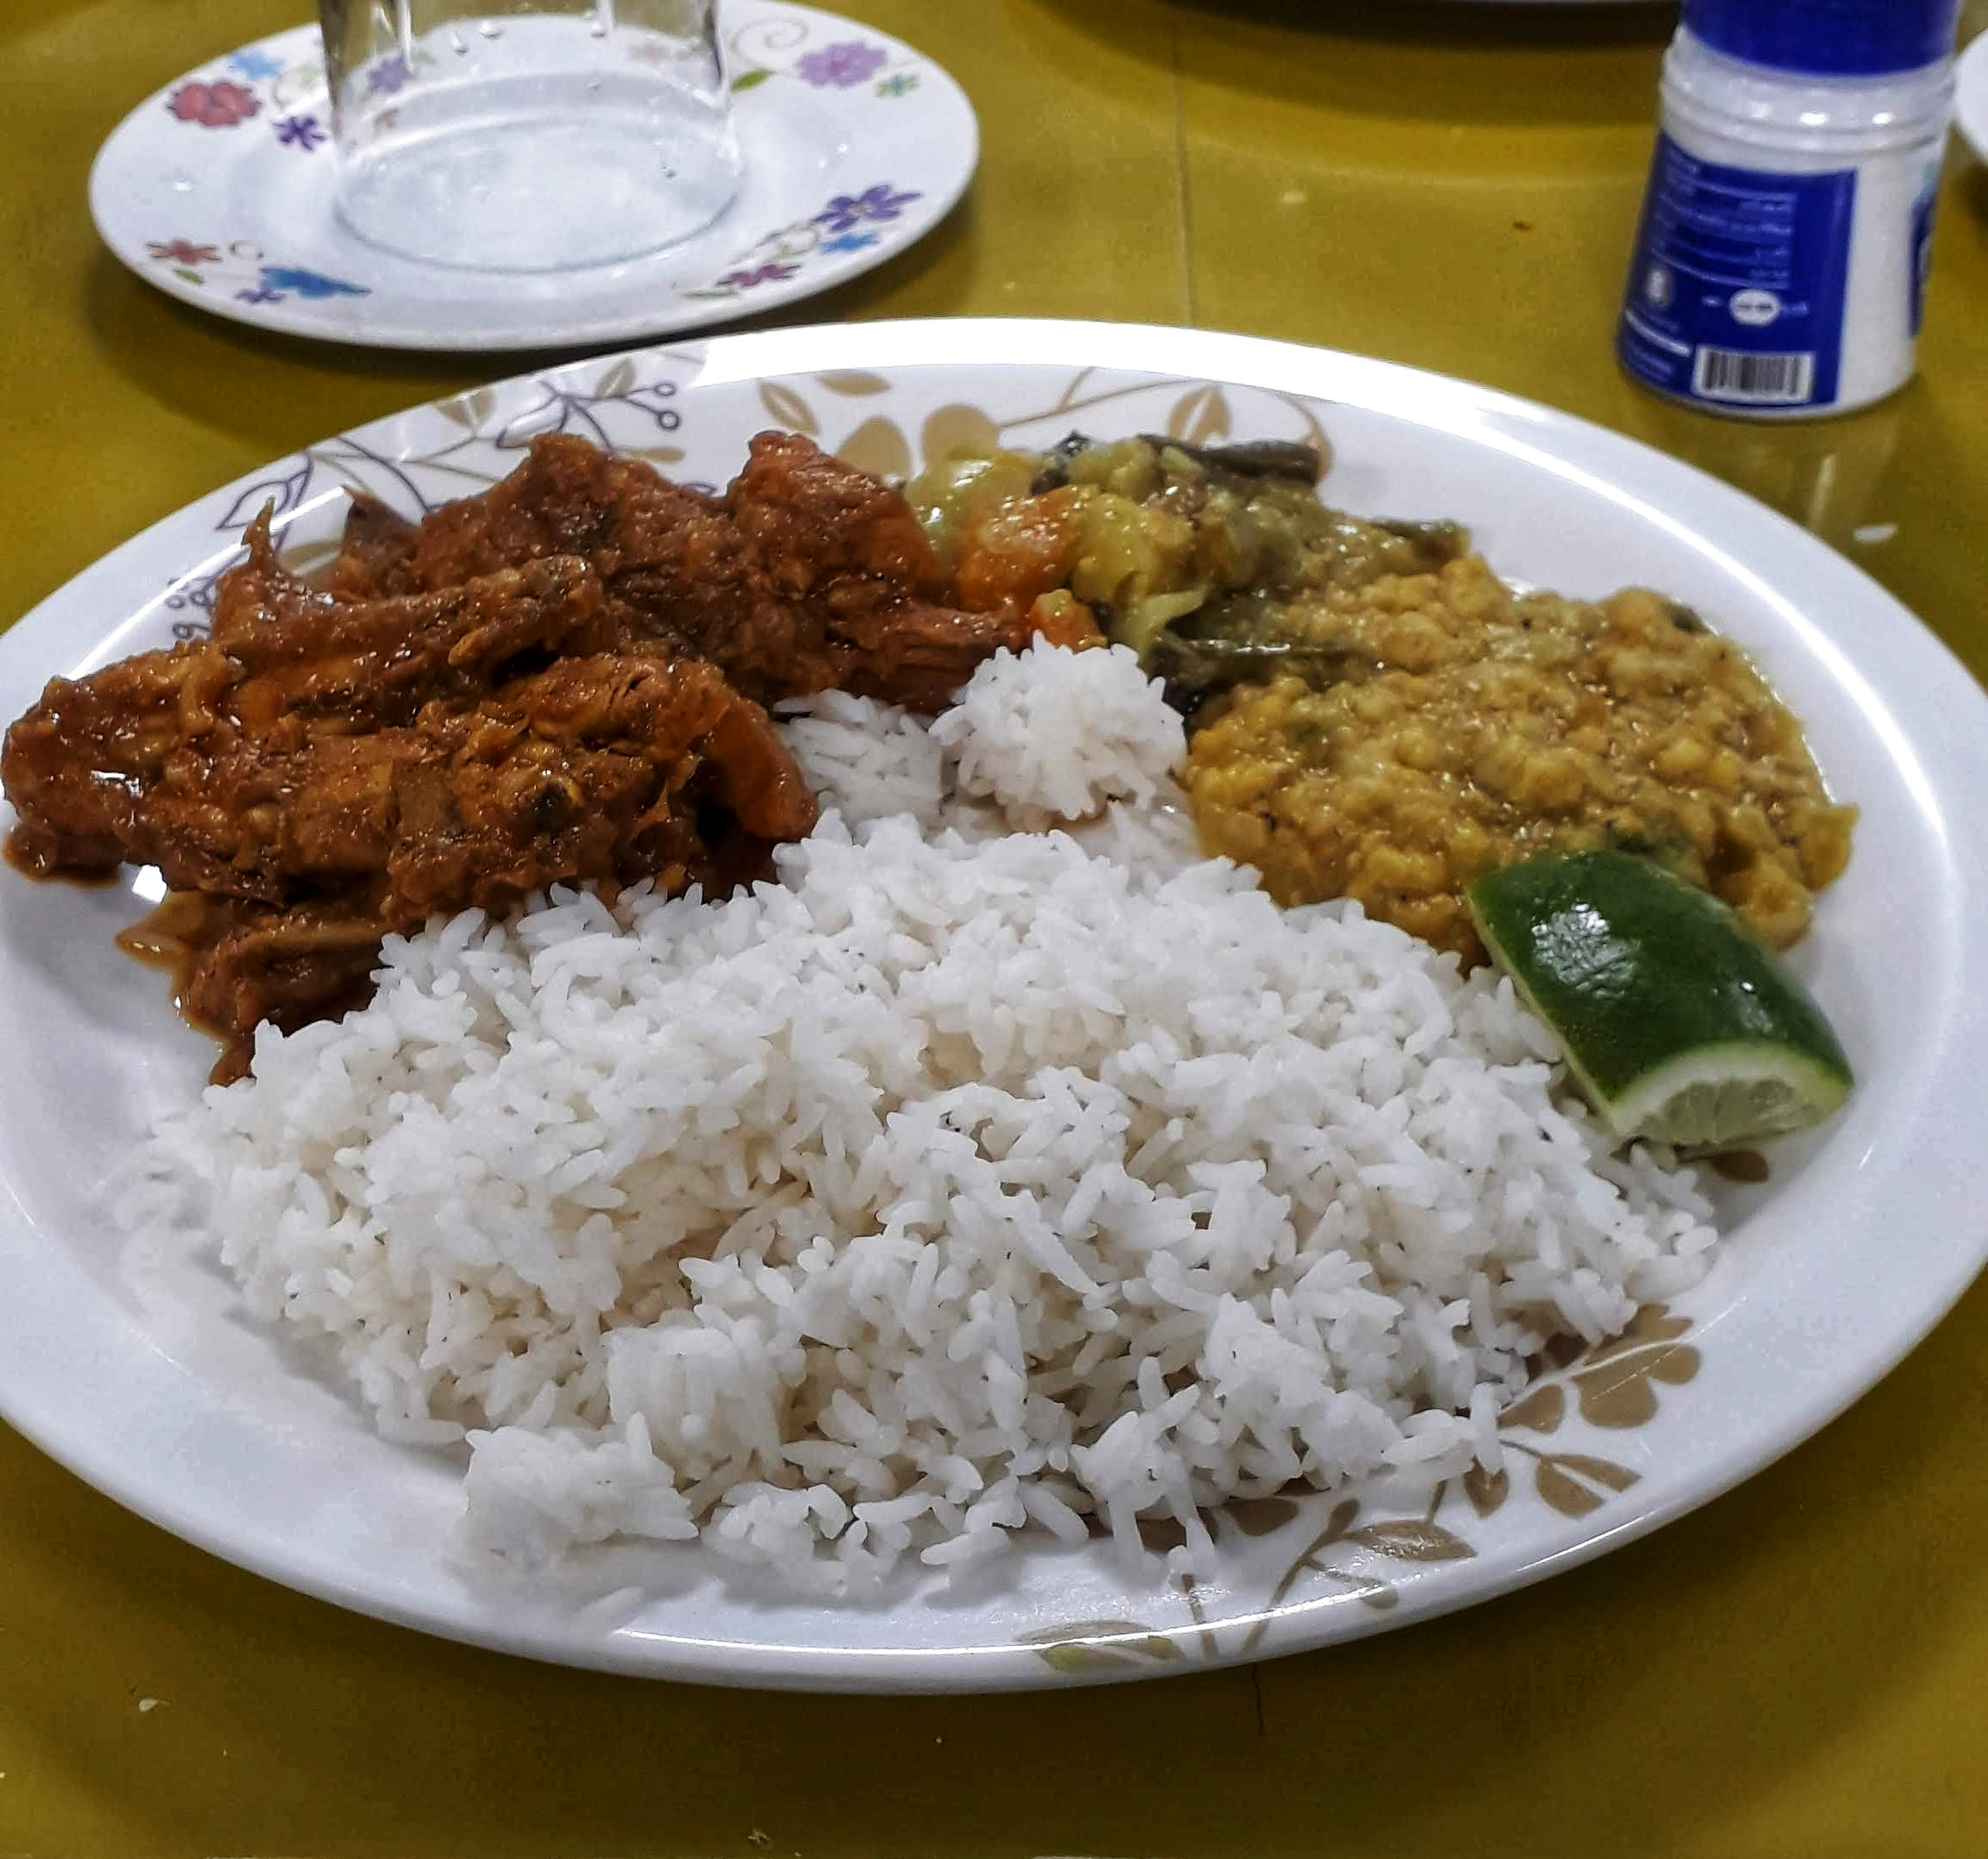
\includegraphics[width=4.6cm]{figures/context/meal_platter.jpg}};
\node[flnote,text width=4.6cm] at (2.35,-2.4) {可见食物与外观提供视觉线索\\实际重量和营养需要估计};

\node[fltrain,anchor=north west,text width=8.7cm,align=left,inner sep=8pt] (caption) at (6.0,2.9)
 {\textbf{\color{FLBlue}任务一 · 英文描述示例}\\[4pt]
 A plate of white rice with several side dishes.};
\node[flaccent,anchor=north west,text width=8.7cm,align=left,inner sep=8pt] (record) at (6.0,1.15)
 {\textbf{\color{FLBlue}任务二 · JSON 字段示例}\\[4pt]
 {\ttfamily\fontsize{8.5}{10.5}\selectfont
 \{\\
 \hspace*{1em}"items": [\{"name": "rice", "weight\_g": null\}],\\
 \hspace*{1em}"total\_weight\_g": null,\\
 \hspace*{1em}"total\_calories\_kcal": null,\\
 \hspace*{1em}"protein\_g": null,\\
 \hspace*{1em}"fat\_g": null,\\
 \hspace*{1em}"carbohydrate\_g": null\\
 \}}\\[4pt]
 {\fontsize{8}{10}\selectfont\color{FLMid}仅列一项食材；null 表示待估，实际输出须为数值。}};
\draw[flarrow] (4.72,.95) -- ++(.55,0) |- (caption.west);
\draw[flarrow] (4.72,-.6) -- ++(.55,0) |- (record.west);

\draw[FLLine,dashed] (0,-3.65)--(15.25,-3.65);
\node[fllabel,anchor=west] at (0,-4.0) {训练衔接：描述模型如何成为 Hybrid};
\node[flnode,text width=3.7cm,minimum height=.85cm] (source) at (2.05,-4.85)
 {任务一训练好的模型 A\\图像描述能力};
\node[flaccent,text width=4.65cm,minimum height=.85cm] (transfer) at (7.6,-4.85)
 {迁移视觉编码器与 GRU\\新增重量、营养回归头};
\node[fltrain,text width=3.7cm,minimum height=.85cm] (hybrid) at (13.15,-4.85)
 {任务二数据联合训练\\得到 Hybrid 模型};
\draw[flarrow] (source.east)--(transfer.west);
\draw[flarrow] (transfer.east)--(hybrid.west);
\end{tikzpicture}


\caption{餐食输入、两类输出示例与 Hybrid 的训练衔接。文字和字段为人工示意，非模型预测；null 为待估占位，实际预测需填入数值。}
\label{fig:meal-evidence}
\vspace{2pt}
{\scriptsize\color{FLMid}照片：Sm faysal，\href{https://commons.wikimedia.org/wiki/File:Plain_rice_chicken_vegetables_lintel_\%26_lemon_lunch_platter_from_Bangladesh.jpg}{Wikimedia Commons}，\href{https://creativecommons.org/licenses/by-sa/4.0/}{CC BY-SA 4.0}；仅等比例缩放。}
\end{figure}

\subsection{相关研究基础与关键困难}
\textbf{从全局概括到局部辨识。}经典图像描述方法建立了视觉编码与语言生成的联系，空间注意力进一步使模型在生成不同词语时读取不同区域\cite{vinyals2015show,xu2015attend}。Food-500 Cap 将评价落到菜品、可见食材和属性等细粒度内容\cite{ma2023food}。但烹饪改变外观、配料占比小和相互遮挡，使主要菜品正确而局部细节遗漏成为需要单独分析的问题。本项目据此比较全局与网格表示，并用消融实验辅助解释空间信息的作用。

\textbf{从食材语义到定量记录。}Inverse Cooking 研究图像中的食材预测及其与语言生成的联系，Nutrition5k 则以物理测量和营养标注支持份量与营养估计\cite{salvador2019inverse,thames2021nutrition}。二者提示，回答“有什么”与“有多少”需要不同监督。单张 RGB 图像缺少可靠尺度，投影面积也不能确定厚度、密度与遮挡份量；油脂等隐含成分进一步增加误差。本项目将食材生成与数值回归结合，分别评价识别错误与定量偏差，不将视觉上合理的输出视为真实测量。

\textbf{从文本相似到图像事实。}同一餐食可以有多种正确描述，而 Food-500 Cap 每图只有一条参考，词语重合指标对合理改写的覆盖有限。生成模型还可能依据常见搭配补出图中缺乏证据的食材。CLIPScore、FLEUR 等研究提供了直接结合图像评价描述的思路\cite{hessel2021clipscore,lee2024fleur}，但自动评价仍需检查其判断偏差。因此，本项目同时分析传统指标、视觉条件 Judge 与人工评分，检验指标提升是否伴随事实质量改善。各研究路线的详细比较见第~\ref{sec:related-work}~节。

\subsection{研究问题与任务设置}
\textbf{任务一：空间信息是否有助于食物细节描述？}在 Food-500 Cap 上自主实现两种课程指定结构：模型 A 采用 ResNet-18 全局表示与 GRU，模型 B 采用 ResNet-18 网格表示与 Transformer 编解码器。统一图文划分、词表规则和贪心解码，报告 BLEU-4、METEOR、ROUGE-L、CIDEr-D。A/B 比较反映两条路线的整体差异；另设保留 B 编解码配置、仅压缩视觉输入的 B-global，辅助分析空间信息贡献，并检查同图输出中的食材遗漏与属性误识别。

\textbf{任务二：描述模型的迁移与预训练模型的领域适配各有何收益？}采用教学云平台数据，保留训练、验证、测试的原始划分，分别为 2\,338、414、506 条。自主路线将 A 的视觉与序列参数迁移到 Hybrid，生成食材名称及对应重量，并独立回归整餐总重量、热量、蛋白质、脂肪和碳水化合物，组装为统一 JSON。通过“仅视觉迁移”与“视觉加 GRU 迁移”比较序列参数复用的作用。预训练路线拟采用 Qwen3-VL-4B-Instruct 与 LoRA，在相同基础版本、输入和解码条件下比较适配前后，再与 Hybrid 对照\cite{hu2022lora}。两条路线均报告任务一文本指标、食材名称 F1 和数值 MSE，补充逐字段误差及 Schema 有效率；质量单位为 g，热量单位为 kcal。

\textbf{选做实验：奖励优化的收益是否与视觉事实一致？}本组选择 SCST 与 Judge 两个方向，均纳入交付。SCST 从选定的 A 交叉熵权重出发，以 CIDEr-D 为奖励，并与原始交叉熵版本及等步数继续交叉熵版本比较\cite{rennie2017scst}。Judge 对匿名描述的语义正确性、内容覆盖、幻觉和流畅度评分，再与双人独立评分及传统指标对照。实验检验收益及其局限，不预设奖励提升必然减少幻觉。

\subsection{预期贡献与研究边界}
本项目的设计特色体现在三个可检验的方面：一是将描述模型的视觉与序列能力迁移到结构化膳食任务，通过迁移对照检验复用价值；二是在完整食材名称的生成边界对齐重量预测，结合独立整餐回归形成语义与数值联合输出，并分解其错误来源；三是将序列奖励优化与图像事实评价结合，分析自动指标和人工判断之间的一致与分歧。上述内容属于面向课程任务的结构设计与实验探索，效果由后续实验验证，具体实现见第~\ref{sec:technical-plan}~节。

食堂是应用动机，当前结论限定于指定数据与划分，尚不能据此宣称对校园真实餐食的泛化效果。Food500 图文需经可追溯映射、哈希与重复组核验后固定清单；词表、数值统计和奖励统计仅由训练集拟合，验证集用于选模。测试前冻结模型与评价协议，推理只读取 RGB、必要的样本标识和固定指令；评价保留缺失、截断及解析失败，以全部目标样本为分母。正式训练效果与 GPU 资源数据均有待实测。


\clearpage
\fancyhead[R]{\small\color{FLMid} 相关工作}
\setcounter{section}{3}
% V3 reusable chapter. Load graphicx and figures/figure_style.tex in the host preamble.
\section{相关工作}
\label{sec:related-work}

食物图像理解包含两个相互关联的目标：将可见内容转化为自然语言，以及将食材组成、份量与营养信息组织为膳食记录。围绕这两个目标，相关研究逐步形成了从视觉表示、序列生成到领域适配和质量评价的方法体系。本节沿四条研究主线梳理代表性进展，为 FoodLens 的自主模型实现与预训练模型适配提供依据。

\subsection{食物图像描述生成研究}
\label{subsec:captioning}
\flfocus{视觉表示由全局向量走向空间 Token，信息交互由循环状态走向注意力与跨层融合。}

\subsubsection{从全局视觉表示到空间注意力}
\textbf{Show and Tell}\cite{vinyals2015show} 将视觉识别与语言生成统一为条件序列建模：预训练 CNN 提取全局图像向量，LSTM 根据图像条件与历史词语逐词生成描述，通过最大化参考句子的条件似然训练。图像在初始时间步输入，后续信息由循环状态传递。该工作在多个数据集上验证了 \textbf{CNN--RNN 编解码范式}，在其 MS COCO 开发集设置下取得 27.7 的 BLEU-4，为从图像到语言的端到端建模建立了清晰起点。

全局向量适合概括场景，食物描述则经常依赖分散的配料、颜色和形态。将整张图像压缩为单一表示，容易弱化多个局部对象及其细微属性。FoodLens 的 \textbf{ResNet-18 + GRU} 延续这一视觉编码与循环解码思路，以轻量骨干和门控循环单元构建自主基线；其设计重点是建立可解释的编码、条件注入和自回归生成流程。原始 Show and Tell 采用 LSTM，GRU 是课程项目对循环解码器的具体选择。

\textbf{Show, Attend and Tell}\cite{xu2015attend} 通过空间注意力将局部视觉信息引入逐词生成。模型保留 VGG-19 的 $14\times14\times512$ 特征网格，根据前一时刻的解码状态计算区域权重，形成动态视觉上下文。软注意力采用可微的区域加权和，硬注意力通过位置采样与随机梯度估计训练。二者都围绕“生成当前词语时关注哪些区域”建立视觉与语言的联系，注意力热图直观呈现这种对应关系。

该论文在 Flickr8k、Flickr30k 和 MS COCO 上验证了注意力机制，软、硬注意力在不同指标上各有优势。\textbf{双随机注意力正则项}鼓励句子生成过程覆盖不同区域，门控系数则调节视觉上下文的使用程度。空间选择缓解了全局压缩的信息瓶颈，也促使后续方法进一步研究区域之间的关系和不同层次视觉信息的组织方式。

\subsubsection{Transformer 与网格特征建模}
Transformer 图像描述模型通过\textbf{自注意力与交叉注意力}连接视觉表示和文本生成：视觉自注意力组织位置之间的关系，文本掩码自注意力建模历史词语，交叉注意力读取视觉上下文。网格特征将卷积特征图组织为视觉 Token，保留局部区域信息，再结合位置表示建模空间关联。训练时各词位置可在给定真实前缀的条件下并行计算，推理时采用自回归生成。

\textbf{Meshed-Memory Transformer}\cite{cornia2020meshed} 同时改进视觉编码和跨层解码。编码器引入可学习的持久记忆向量，解码器通过带门控的网状连接读取多个编码层，从而综合不同层次的区域关系。论文在 COCO Karpathy 划分及在线评测中报告了性能改进。该方法主要采用检测区域特征，其“网状”结构指编码层与解码层之间的连接，为利用多层视觉信息提供了代表性思路。

\textbf{S$^2$ Transformer}\cite{zeng2022s2} 将这一问题推进到网格特征的空间与层次建模。其空间感知伪监督模块（Spatial-aware Pseudo-supervised，\textbf{SP}）学习聚类中心，对网格进行软分配，并聚合相对于中心的残差，形成伪区域特征。原始网格与伪区域由共享参数的编码器处理，在局部覆盖和聚合语义之间形成互补，整个过程使用可学习聚类而无需额外区域标注。

其尺度增强模块（Scale-wise/Scale-aware Reinforcement，\textbf{SR}）拼接不同编码层的输出，经映射与加权残差补充最高层表示，再融合两个分支供解码器使用。SR 的作用是跨层特征融合，序列级奖励训练由独立的训练阶段完成。论文采用来自预训练检测器的 $7\times7\times2048$ 网格输入。在相同 ResNeXt-101 特征、MS COCO Karpathy 测试划分及论文两阶段训练协议下，加入 SP 和 SR 后，CIDEr 由 131.2 提升至 133.5，表列参数量由 33.57M 增至 34.64M，展示了空间聚合与层次融合的收益。

图\ref{fig:s2-architecture}展示 S$^2$ 的实际网络：左侧网格与右侧伪区域经过共享编码，底部 SP 完成空间聚合，两侧 SR 将多层信息补充到解码表示。表\ref{tab:captioning}进一步比较各方法的技术重点。FoodLens 据此设置\textbf{全局特征 + GRU}与\textbf{空间网格 + Transformer}两种自主模型，考察局部信息与注意力建模对食物描述的影响。S$^2$ 为网格模型提供设计依据，M$^2$ 提供多层信息利用的参照；项目比较时结合视觉表示和解码结构两个变化解释结果。

\begin{figure}[!htbp]
 \centering
 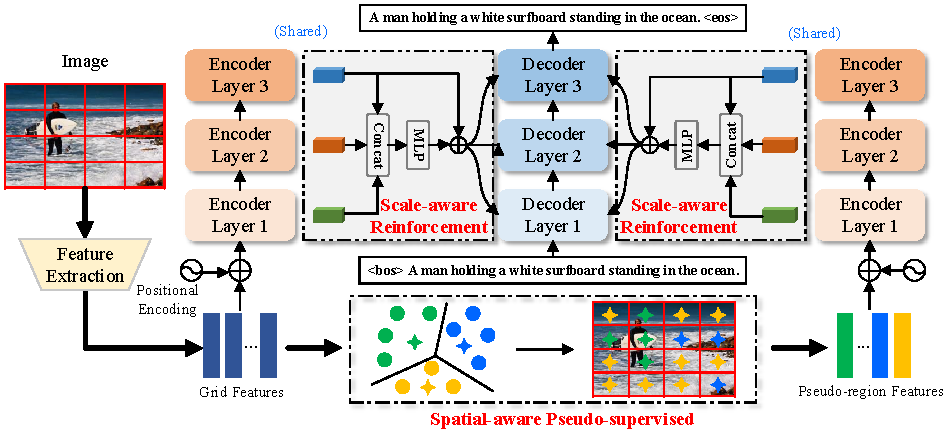
\includegraphics[width=\linewidth]{figures/literature/s2-fig2.pdf}
 \caption{S$^2$ Transformer 的网格与伪区域双分支架构。引自 Zeng 等\cite{zeng2022s2}\href{https://www.ijcai.org/proceedings/2022/0224.pdf}{原图 2（IJCAI）}，裁去页面正文，保留原图连接。SP 聚合网格，SR 融合编码层。}
 \label{fig:s2-architecture}
\end{figure}

\begin{table}[!htbp]
 \caption{图像描述模型的表示与生成方式比较}
 \label{tab:captioning}
 \centering\small
 \setlength{\tabcolsep}{5pt}\renewcommand{\arraystretch}{1.16}
 \begin{tabularx}{\linewidth}{@{}P{3.0cm}P{3.1cm}P{3.15cm}Y@{}}
 \toprule
 \textbf{方法} & \textbf{视觉表示} & \textbf{解码与交互} & \textbf{技术特点}\\
 \midrule
 Show and Tell & CNN 全局向量 & LSTM 循环生成 & 简洁的条件序列基线\\
 Show, Attend and Tell & CNN 空间网格 & 注意力 + LSTM & 逐词选择视觉区域\\
 M$^2$ Transformer & 检测区域、多层编码 & 记忆增强、网状跨层解码 & 综合多层区域关系\\
 S$^2$ Transformer & 原始网格、SP 伪区域 & 共享编码、SR 融合 & 空间聚合与层次互补\\
 \bottomrule
 \end{tabularx}
\end{table}

\subsubsection{细粒度食物描述与领域适配}
\textbf{Food-500 Cap}\cite{ma2023food} 将图像描述评价推进到细粒度食物领域。研究从 ISIA Food-500 的 494 个类别中各选择 50 张图像，共构建 24,700 个图文样本。每张图像对应一条人工描述，覆盖菜品名称、可见食材、颜色、形状和容器，并为类别补充饮食文化来源标签。这类标注将“识别菜品”扩展为“描述区分菜品的可见细节”，与 FoodLens 的任务一直接对应。

该研究以分类、检索、描述和图像合成四种零样本任务探测九种视觉语言模型。描述评价使用 BLEU、METEOR、ROUGE、CIDEr、CLIPScore，以及检查类别名称的\textbf{语义标签准确率}。实验揭示了食物属性遗漏、误识别和不同饮食文化类别的表现差异，说明领域适配与细粒度分析具有实际价值。每图单参考对合理改写的覆盖有限，类别名称匹配侧重菜品识别；FoodLens 因而结合自动指标与食材、属性错误分析评价描述质量，重量和营养标签则由结构化膳食任务提供。

\FloatBarrier
\subsection{食物理解与结构化营养估计研究}
\label{subsec:nutrition}
\flfocus{食材集合回答“有什么”，重量与营养估计回答“有多少”；定量预测依赖可靠的份量监督。}

\subsubsection{食材集合识别与依赖关系}
\textbf{Inverse Cooking}\cite{salvador2019inverse} 以“图像理解—食材预测—食谱生成”组织食物语义推断。模型先从图像预测食材集合，再让步骤解码器同时关注图像特征和食材嵌入。食材预测器利用 Transformer 的自回归过程学习共现关系，以跨时间最大池化后的集合损失减少输出排列的影响，并处理结束标记与集合基数。这种\textbf{依赖建模与集合监督}兼顾了食材间联系和标签的无序性。

在筛选后的 Recipe1M 数据上，论文使用 1,488 项食材词表，测试集全局食材 IoU 和 F1 分别达到 32.11 和 48.61。图像与食材共同生成步骤时，测试困惑度为 8.51，优于仅图像条件的 9.66 和仅食材条件的 8.67，验证了\textbf{视觉信息与显式食材语义的互补性}。该研究的输出是食材集合与食谱，隐藏配料和中间识别错误构成主要困难；将其思想用于膳食记录时，逐食材重量及营养值需要相应的定量标签。

图\ref{fig:inverse-architecture}给出了这一路线的网络结构。食材预测器位于图像编码器与食材编码器之间，步骤解码器接收图像和食材两路表示，将食材识别与语言生成连接起来。

\begin{figure}[!htbp]
 \centering
 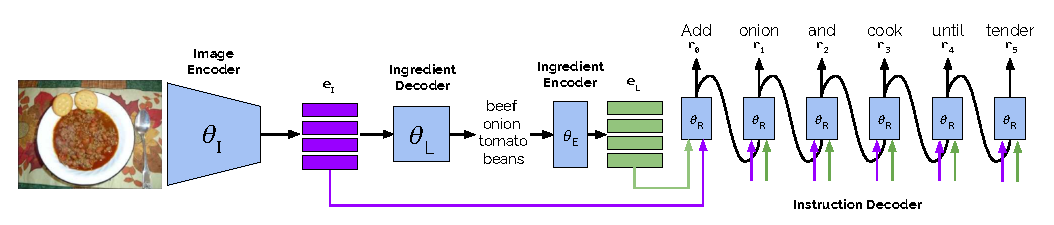
\includegraphics[width=\linewidth]{figures/literature/inverse-cooking-fig2.pdf}
 \caption{Inverse Cooking 的图像、食材与步骤生成网络。引自 Salvador 等\cite{salvador2019inverse}\href{https://openaccess.thecvf.com/content_CVPR_2019/papers/Salvador_Inverse_Cooking_Recipe_Generation_From_Food_Images_CVPR_2019_paper.pdf}{原图 2（CVF）}，仅裁去页面正文；紫色与绿色连接分别传递图像和食材信息。}
 \label{fig:inverse-architecture}
\end{figure}

\subsubsection{份量监督与重量、营养估计}
\textbf{Nutrition5k}\cite{thames2021nutrition} 通过物理测量建立了视觉营养理解的数据基础。论文表 1 列出 5,066 份餐食，涉及超过 250 种食材，约有 20,000 段侧视视频，其中约 3,500 份具有俯视 RGB-D 数据。采集时逐项添加食材或已知配方的成品食物，记录重量增量并扫描；四台侧面摄像机各扫过约 $90^\circ$，共同覆盖餐盘周围视角，俯视 RealSense 提供颜色与深度。

\textbf{增量秤量、配方分解与营养数据库}共同构成标签依据：成品项的食材比例由配方分解，营养值结合食材重量和 USDA 数据库计算。同一餐盘的增量扫描被放入同一数据子集，保持训练与测试之间的餐盘独立性。

Nutrition5k 的主要基线采用 \textbf{InceptionV2 多任务回归}，通过共享视觉特征和任务分支预测热量、宏量营养素以及需要时的总重量，训练与评价主要使用 MAE。论文区分了\textbf{每克营养密度}与\textbf{整餐绝对值}：前者按真实重量归一化标签，并在表中借助真实重量换算为整餐数值；后者直接从 RGB 预测总量，同时承担组成识别与份量估计。数据提供食材级重量，主要回归基线关注整餐级输出。

图\ref{fig:nutrition-architecture}展示共享骨干与多个回归头的连接方式。与图\ref{fig:inverse-architecture}的食材条件生成相比，这一架构将视觉表示直接映射为重量及营养数值，训练监督也相应转向物理测量和数据库标签。

\begin{figure}[!htbp]
 \centering
 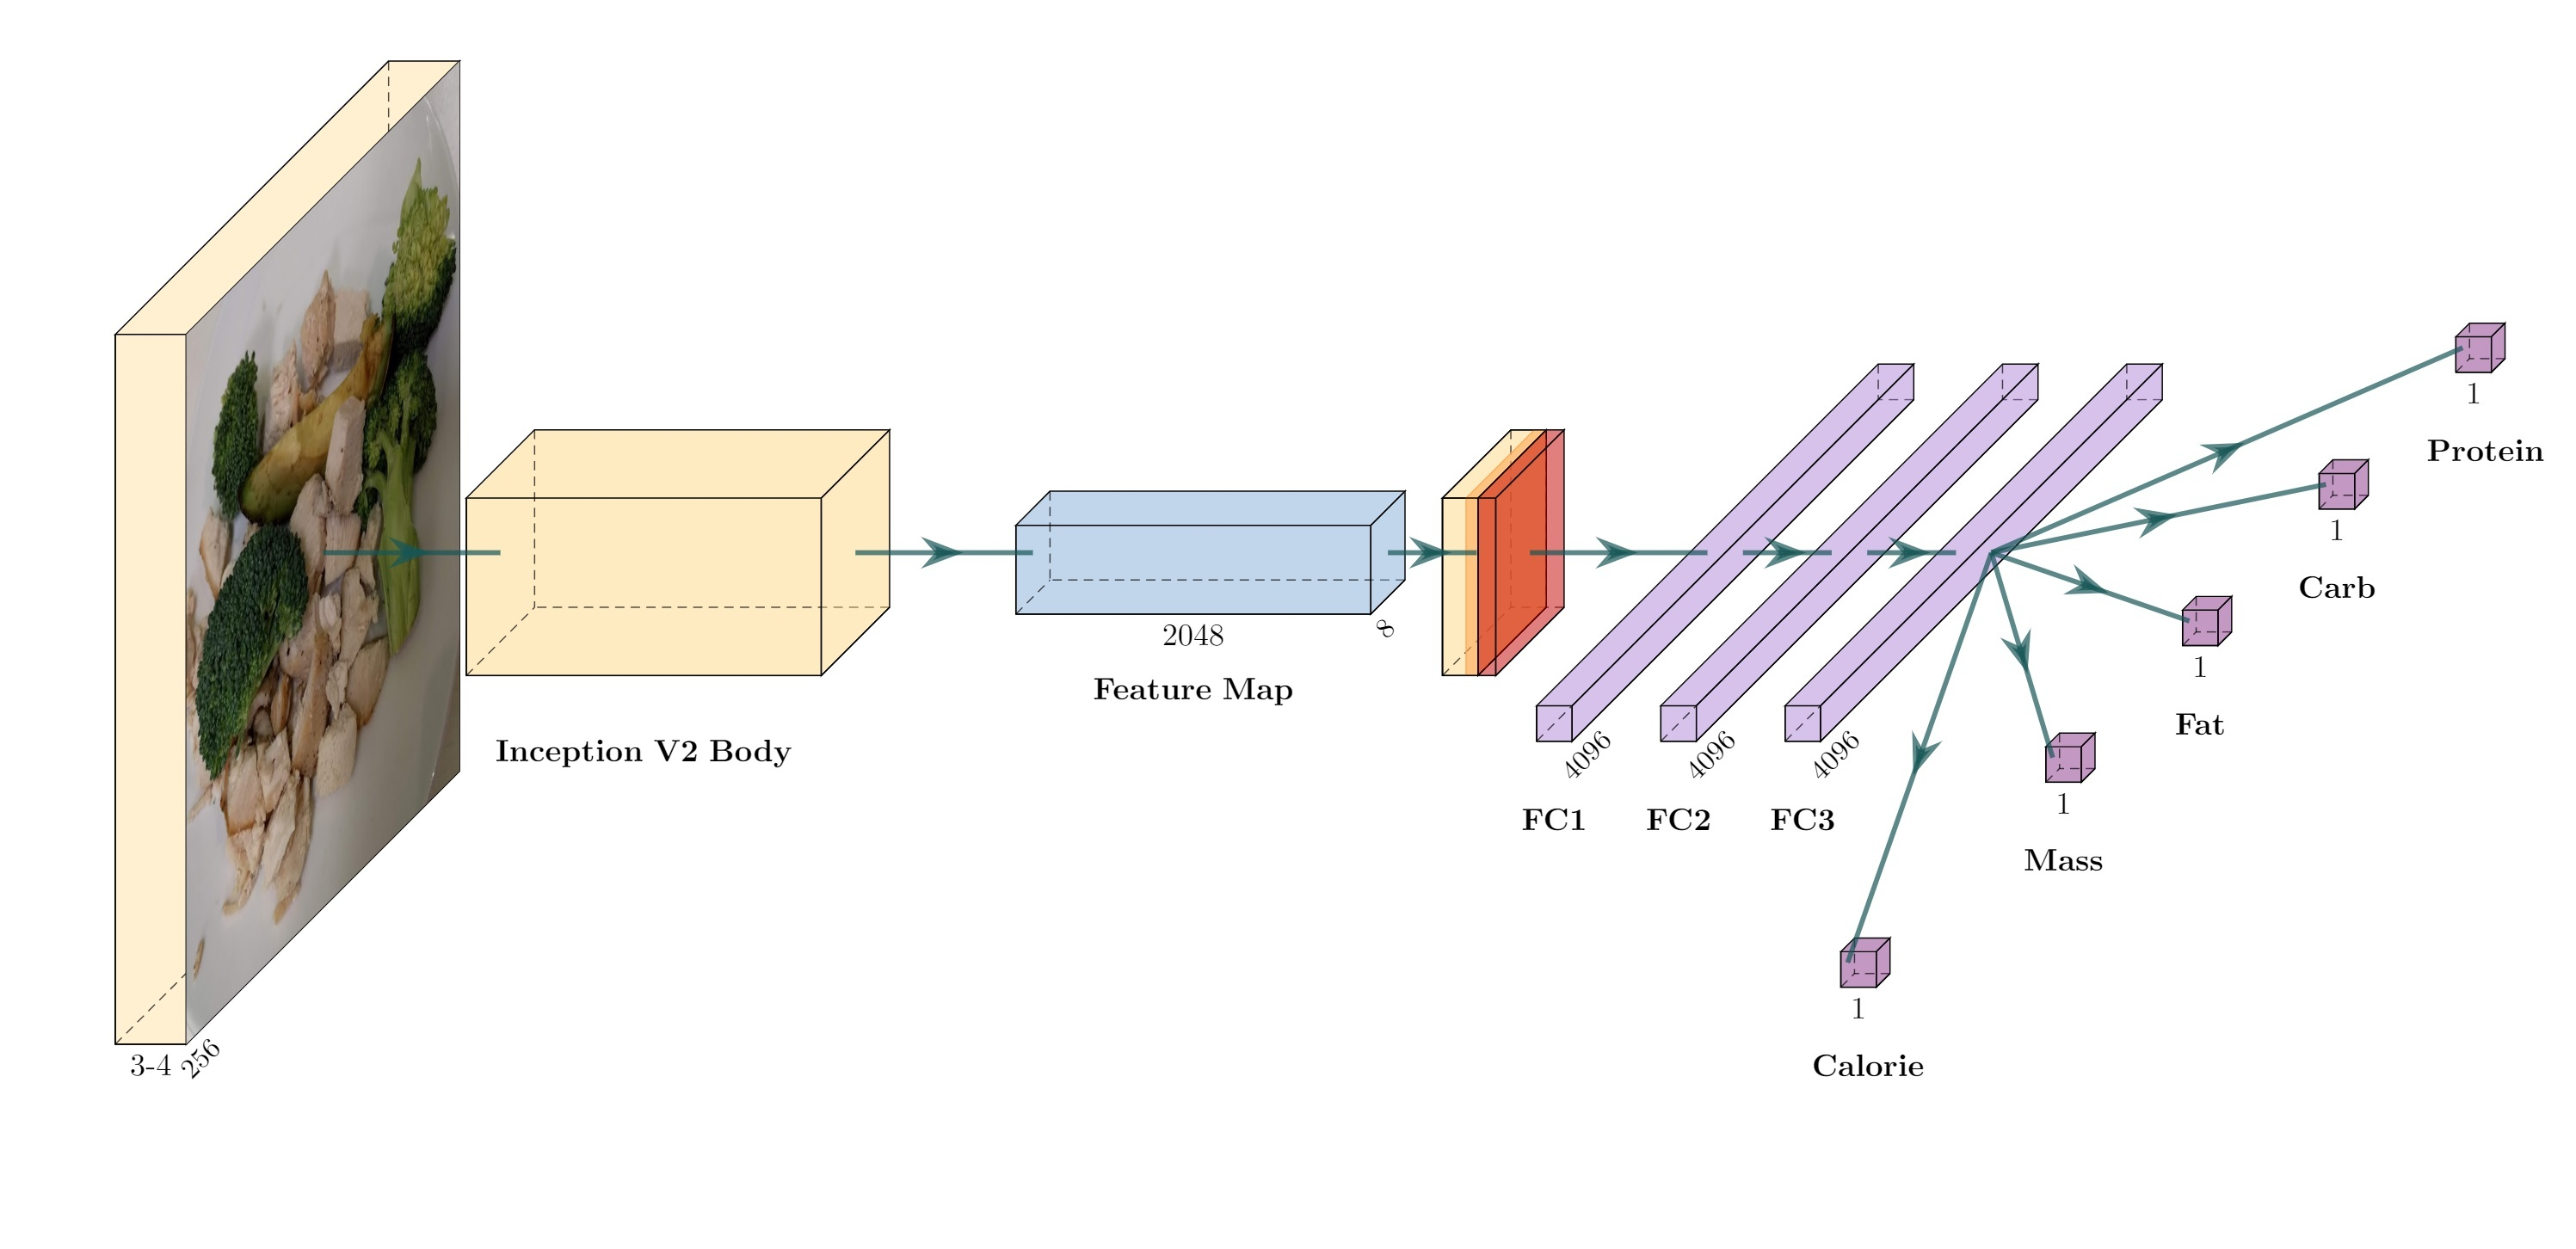
\includegraphics[width=\linewidth]{figures/literature/nutrition5k-fig6.jpg}
 \caption{Nutrition5k 的多任务回归网络。引自 Thames 等\cite{thames2021nutrition}\href{https://arxiv.org/pdf/2103.03375v2}{原图 6}（\href{https://creativecommons.org/licenses/by/4.0/}{CC BY 4.0}）。InceptionV2 后的两层 FC 共享参数，随后以独立分支预测蛋白质、碳水、脂肪、总重量和热量。}
 \label{fig:nutrition-architecture}
\end{figure}

深度信息进一步改善了份量估计。一种设置将深度作为额外通道与 RGB 联合输入；另一种设置根据相机几何和食物前景估计体积，将体积标量与 RGB 特征结合，用独立的 \textbf{InceptionV3 重量网络}预测总重量，再与每克营养密度组合。在论文表 4 的俯视重量回归实验中，图像输入基线 MAE 为 38.1 g，加入体积后降至 29.4 g，显示了几何信息对份量预测的价值。该比较对应相同的重量任务，RGB-D 研究则使用具备深度的子集。

食材组成、份量和营养密度共同决定整餐营养。单张 RGB 图像的主要困难在于尺度缺失、遮挡，以及油脂和调味料等不可见成分；Nutrition5k 集中的采集地点与视角也使跨场景推广成为重要问题。FoodLens 采用课程 RGB 数据，以\textbf{食材 F1、重量与营养 MSE、JSON/Schema 有效率}分别衡量语义、定量和结构质量。这一分层评价将两条研究路线的目标落实到同一膳食记录中，并保留各自明确的检验依据。

\FloatBarrier
\subsection{多模态预训练与参数高效微调}
\label{subsec:vlm-peft}
\flfocus{预训练模型提供图文理解基础，低秩适配与量化分别压缩任务更新规模和基础权重存储。}

\subsubsection{视觉语言基础模型的领域适配}
\textbf{Qwen3-VL}\cite{bai2025qwen} 采用视觉编码器、视觉语言映射模块与 Qwen3 语言模型组成的架构，提供 2B、4B、8B、32B 等稠密模型。其 \textbf{DeepStack} 将多个视觉编码层的特征经专门映射注入语言模型前几层，加强不同层次视觉信息的利用；交错 MRoPE 改进时空位置表示，视频时间戳提供显式时序信息。分阶段预训练与后训练进一步形成多种视觉指令的处理能力。

报告通过视觉问答、文字识别、空间理解和多模态推理基准展示通用能力，并以消融实验支持多层融合的作用。FoodLens 选择 Qwen3-VL 的依据是\textbf{图文理解与指令适配能力}：通过领域样本学习膳食字段和 JSON 输出形式，衔接通用预训练与课程任务。食物重量与营养回归属于领域目标，实际效果由课程数据上的微调前后对照检验。

图\ref{fig:qwen-architecture}呈现基础模型的实际架构：视觉编码器形成视觉 Token，语言模型处理图文序列，右侧 DeepStack 将多个视觉层的特征注入语言模型的早期层。

\begin{figure}[!htbp]
 \centering
 % Original Qwen3-VL Fig. 1 plus an explicitly marked enlargement.
% Main network is unchanged. The video-example region is replaced by the inset.
\begin{tikzpicture}
 \node[inner sep=0,anchor=south west] (original) at (0,0)
  {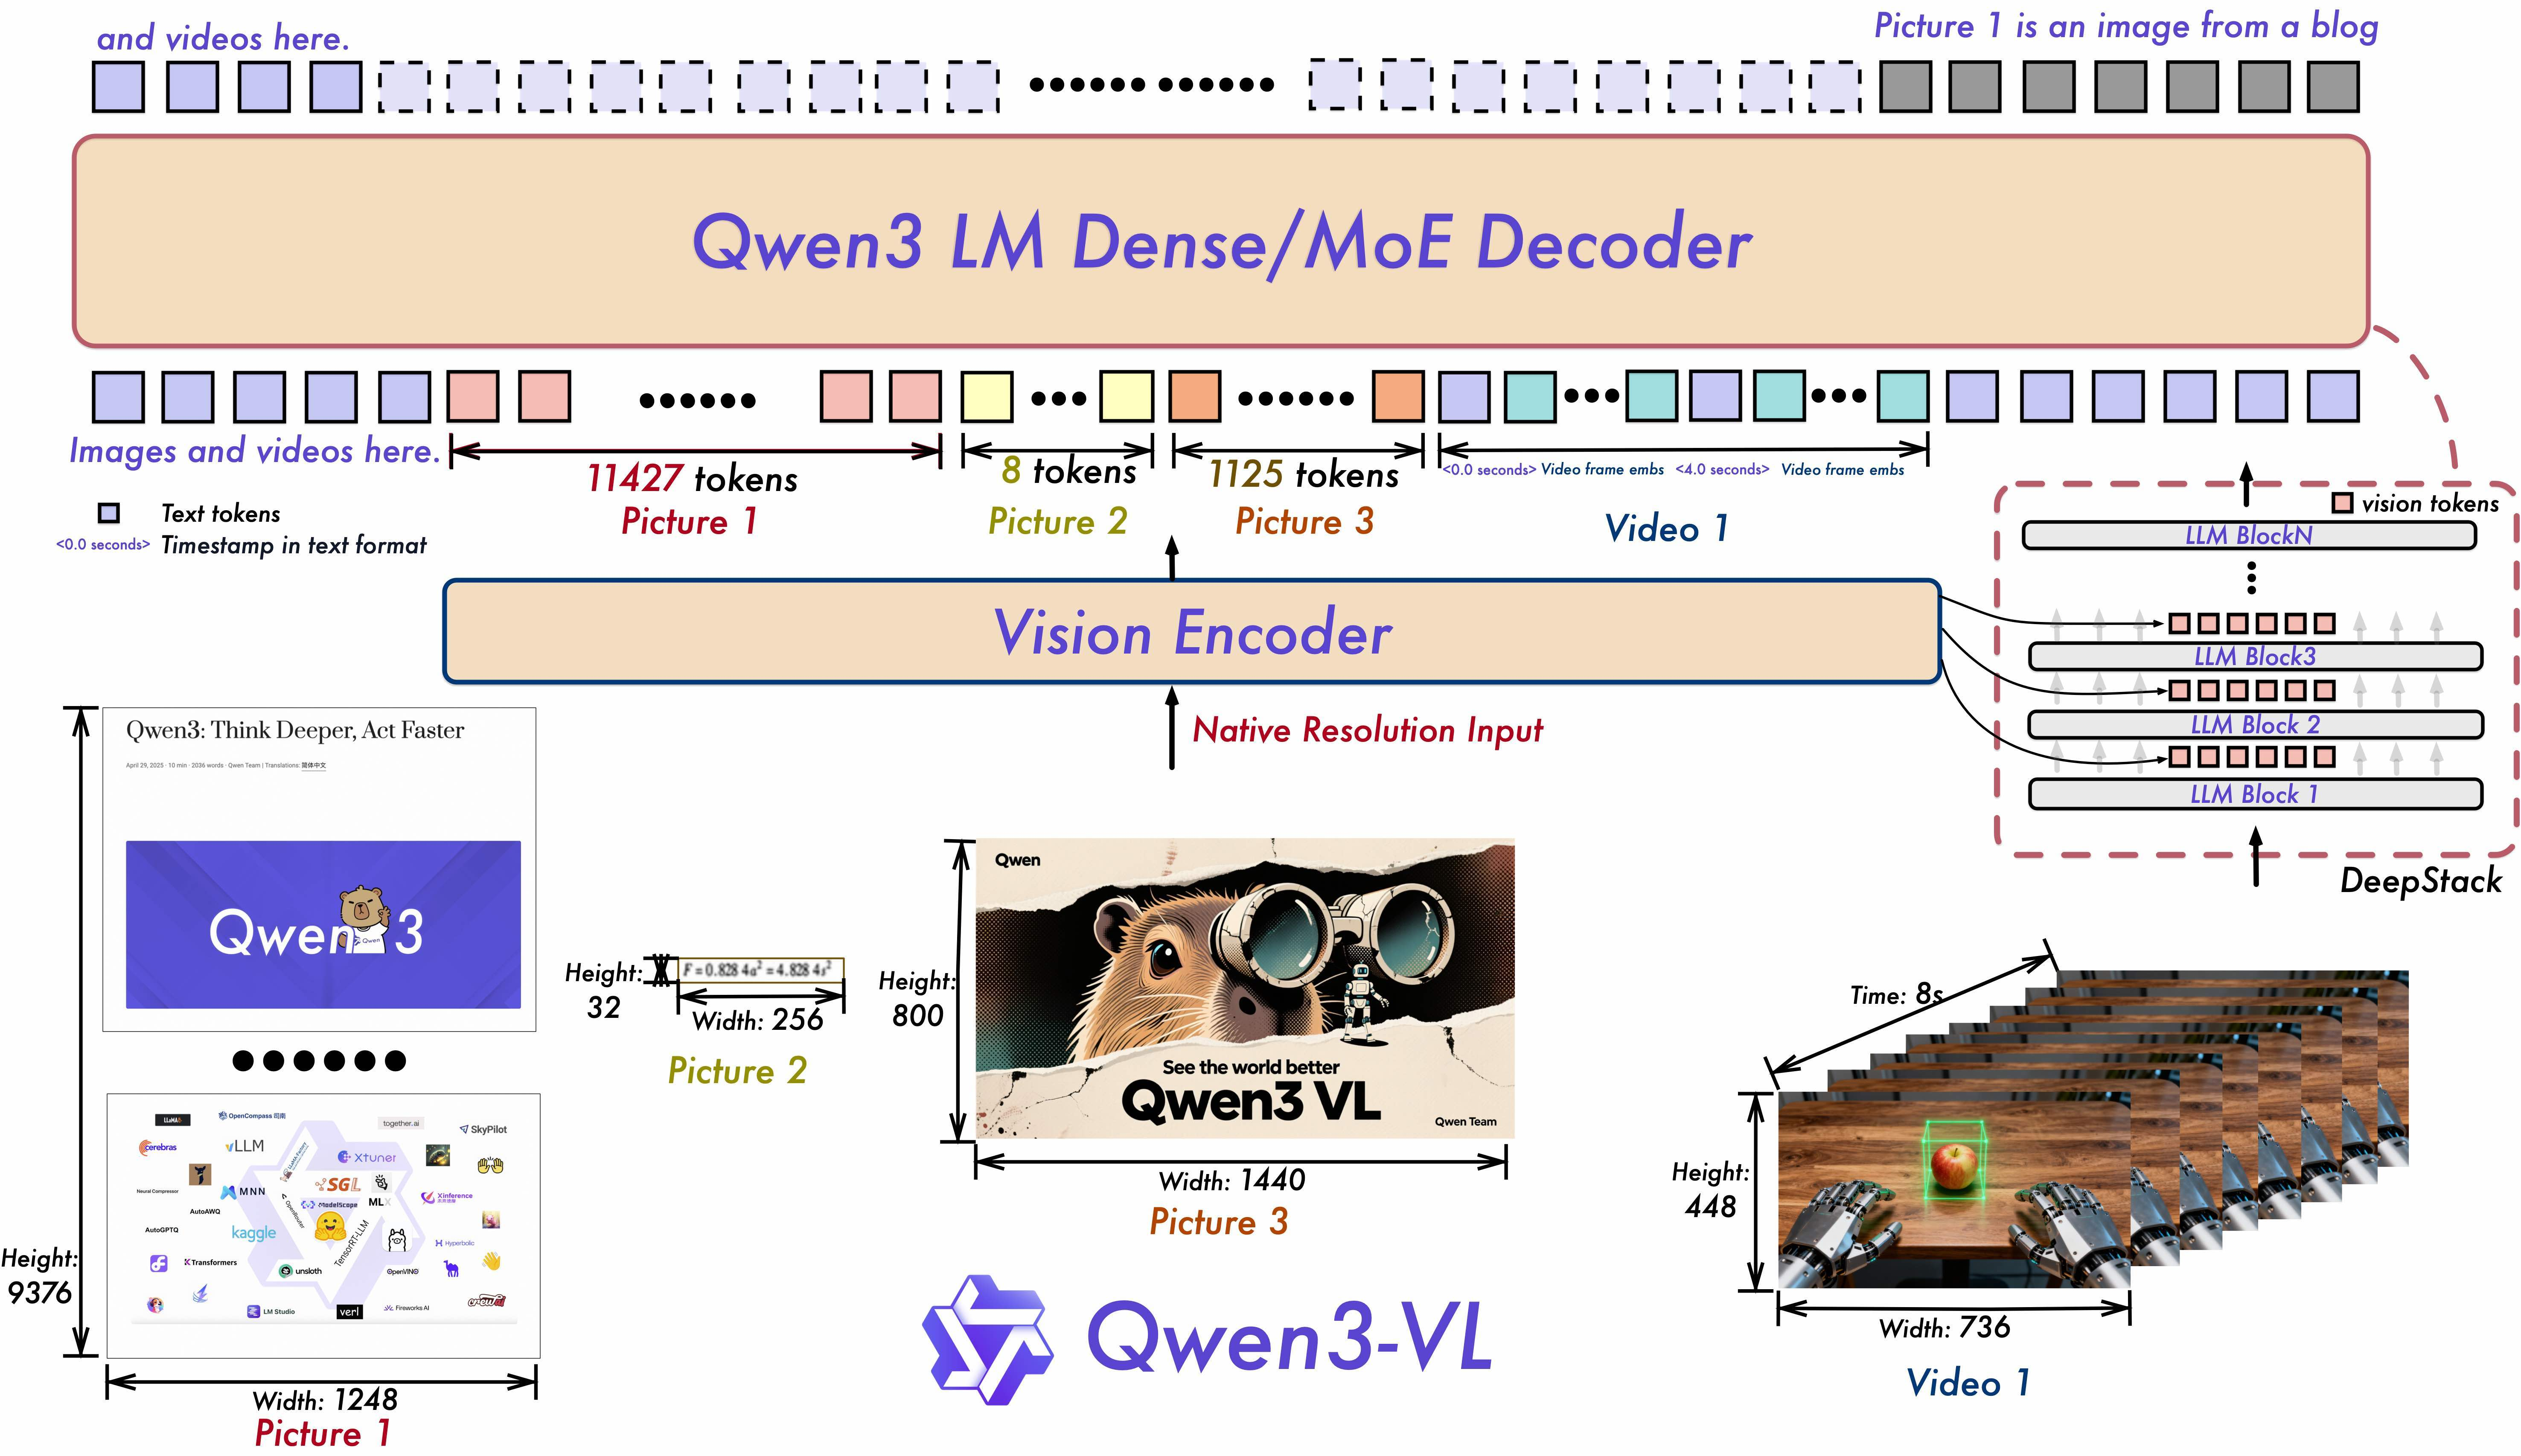
\includegraphics[width=\linewidth]{figures/literature/qwen3vl-fig1.jpg}};
 \begin{scope}[x={(original.south east)},y={(original.north west)}]
  \fill[white] (0.64,0) rectangle (1,0.415);
  \node[anchor=south east,inner sep=0] at (0.998,0.005)
   {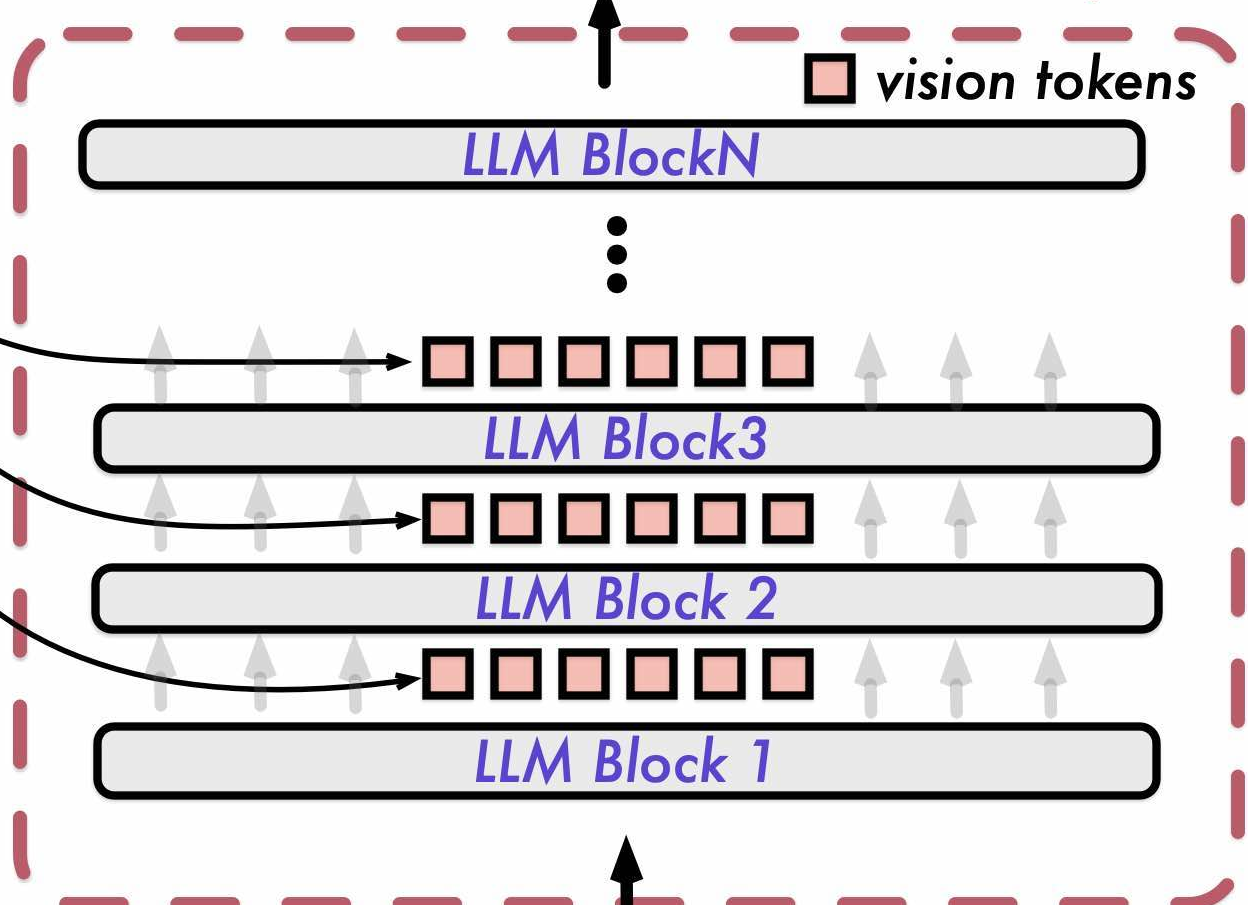
\includegraphics[width=0.30\linewidth]{figures/literature/qwen3vl-deepstack-detail.png}};
  \node[anchor=north,inner sep=0,font=\fontsize{8}{10}\selectfont\bfseries,text=FLBlue]
   at (0.825,0.409) {DeepStack 局部放大};
 \end{scope}
\end{tikzpicture}

 \caption{Qwen3-VL 的多模态基础架构。引自 Bai 等（Qwen Team）\cite{bai2025qwen}\href{https://arxiv.org/pdf/2511.21631v2}{技术报告 v2 原图 1}；右下视频输入示例替换为 DeepStack 局部放大，主体网络与连接保持原样。}
 \label{fig:qwen-architecture}
\end{figure}

\subsubsection{低秩更新与量化存储}
\textbf{LoRA}\cite{hu2022lora} 将任务适配表示为冻结基础权重上的低秩增量。对 $W_0\in\mathbb{R}^{d\times k}$，其更新形式为
\begin{equation}
 W=W_0+\frac{\alpha}{r}BA,\qquad
 B\in\mathbb{R}^{d\times r},\quad A\in\mathbb{R}^{r\times k},
 \quad r\ll\min(d,k).
\end{equation}
可训练参数由 $dk$ 降为 $r(d+k)$，其中 $r$ 控制适配容量，$\alpha$ 调节更新尺度。原论文在多种语言模型任务上获得与全量微调相当或更好的效果，并减少参数、优化器状态及训练显存开销。低秩更新可合入基础权重，便于保存与切换任务适配结果；秩与注入模块共同决定更新范围。

\textbf{QLoRA}\cite{dettmers2023qlora} 在低秩适配基础上，以 4 位形式存储冻结权重，通过反量化参与较高精度计算，将梯度传递给适配器。\textbf{NF4、双重量化与分页优化器}分别优化权重表示、量化常数存储和显存峰值。论文在特定语言模型配置下实现了单张 48 GB GPU 适配 65B 模型，并在多项实验中接近 16 位适配效果；其 33B、65B 与全量 16 位微调的效果比较仍受资源限制。

图\ref{fig:qlora-memory}从基础模型、适配器和优化器状态三个层面比较微调成本。\textbf{LoRA 减少训练更新，QLoRA 进一步压缩基础权重}，共同服务于有限算力下的领域适配。多模态训练的实际成本还取决于视觉 Token 数量、序列长度、模块选择与量化算子兼容性。FoodLens 因而同时记录显存、耗时和任务质量，以食材 F1、数值 MSE 与 Schema 有效率评价微调收益，形成资源效率与领域效果之间的对照。

\begin{figure}[!htbp]
 \centering
 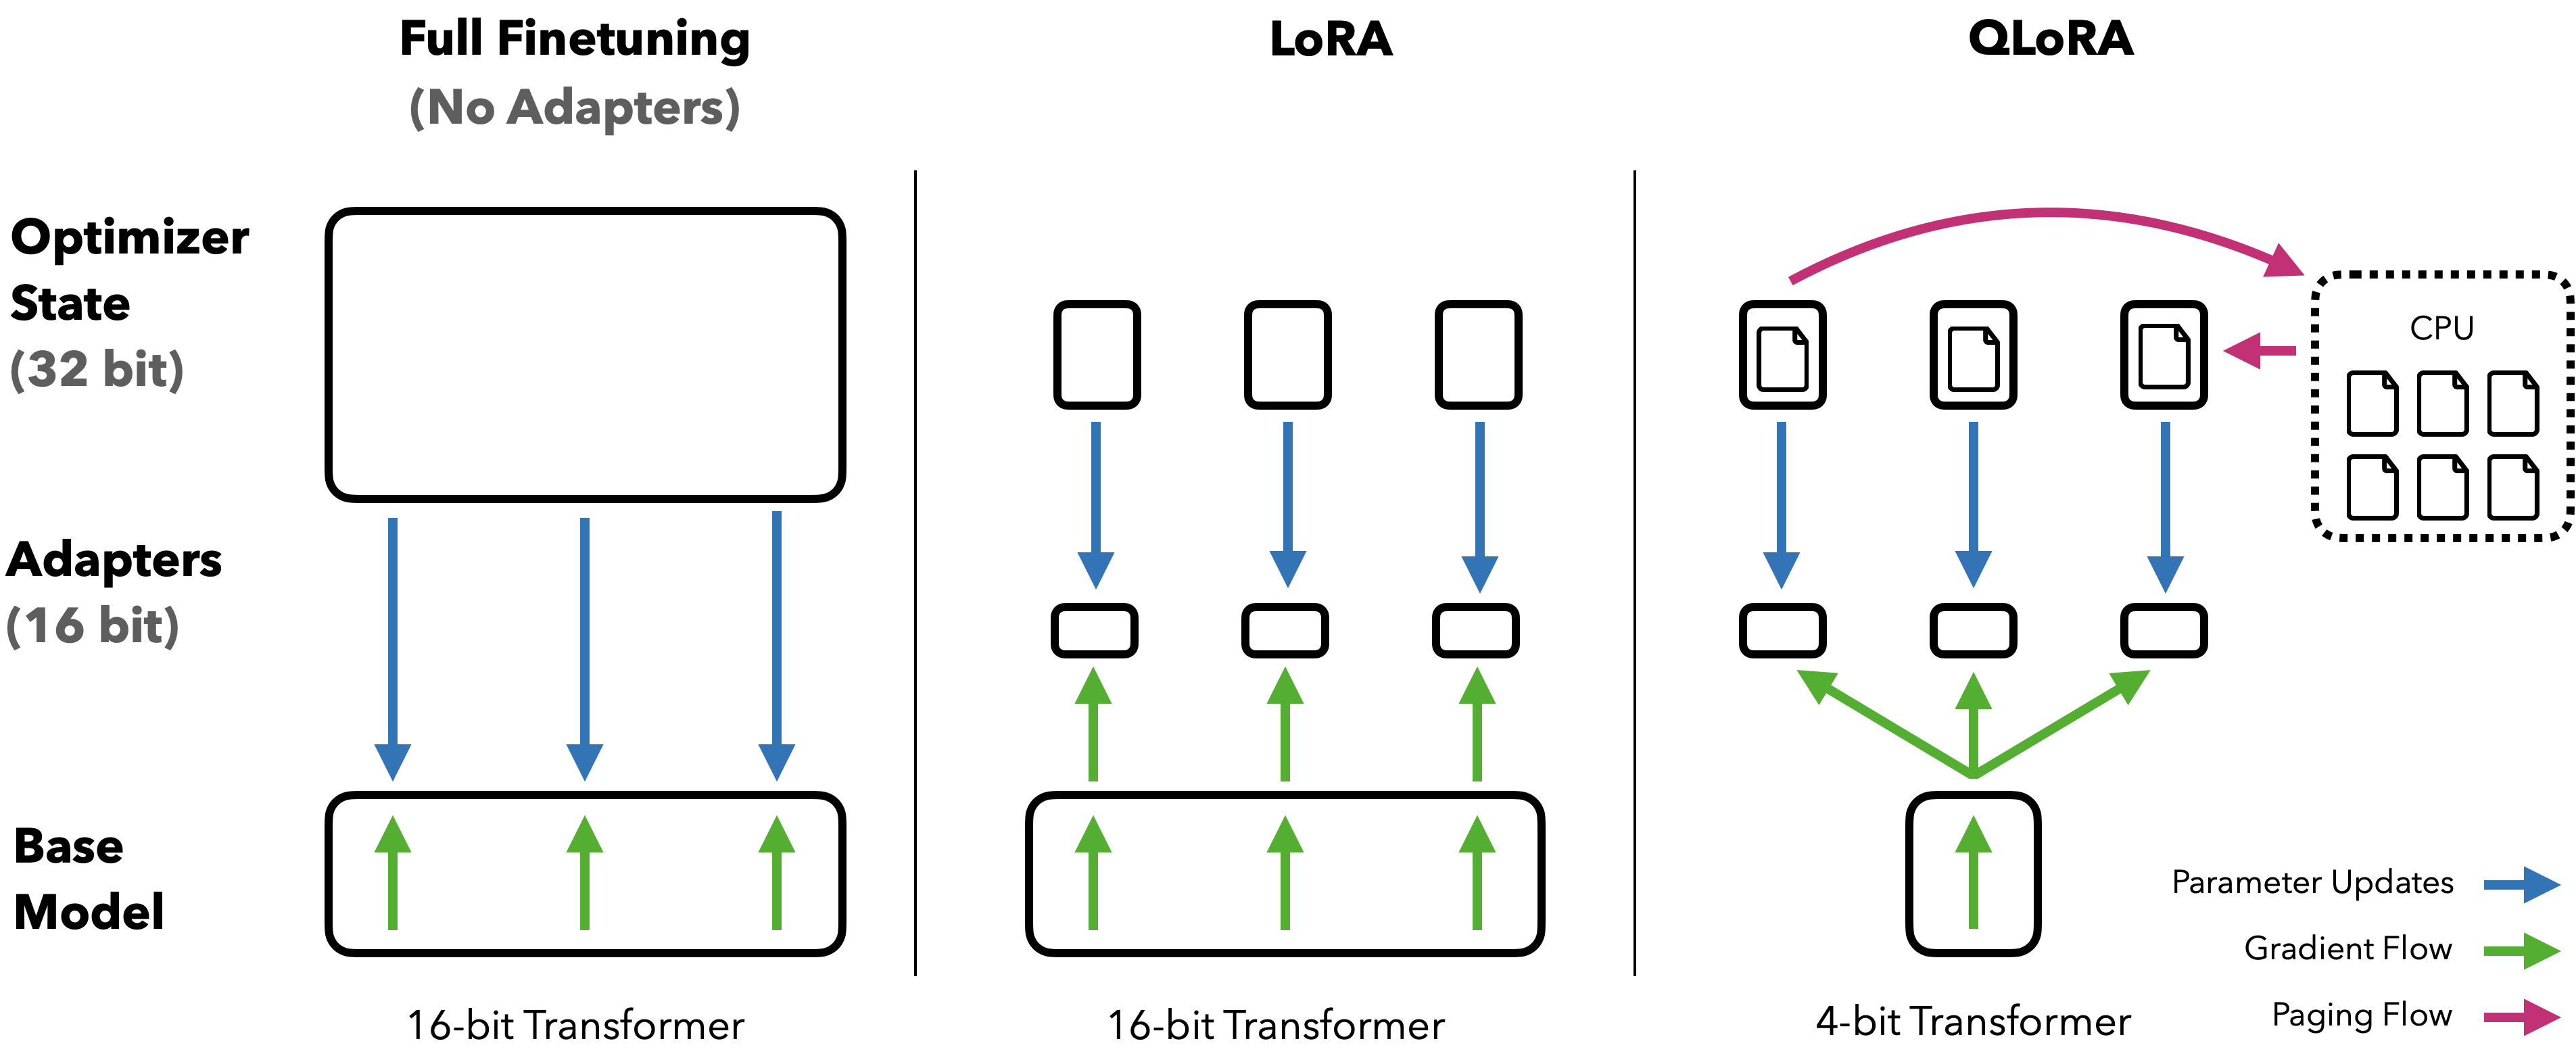
\includegraphics[width=\linewidth]{figures/literature/qlora-fig1.png}
 \caption{全量微调、LoRA 与 QLoRA 的参数更新和存储机制。引自 Dettmers 等\cite{dettmers2023qlora}\href{https://arxiv.org/pdf/2305.14314v1}{原图 1}（\href{https://creativecommons.org/licenses/by/4.0/}{CC BY 4.0}）。QLoRA 冻结 4 位基础权重，以分页优化器缓解显存峰值。}
 \label{fig:qlora-memory}
\end{figure}

\FloatBarrier
\subsection{生成模型的训练优化与评价}
\label{subsec:optimization-evaluation}
\flfocus{训练优化改变模型参数，质量评价检验输出；序列奖励将两者连接起来。}

\subsubsection{从逐词似然到序列级优化}
交叉熵训练逐词拟合参考描述，最终指标则对整句评分；Teacher Forcing 与推理使用自身前缀之间也存在条件差异。\textbf{SCST}\cite{rennie2017scst} 采用策略梯度，将采样描述的奖励与模型自身推理解码结果的奖励之差作为优势信号。经典实现以贪心解码为基线，强化优于当前推理结果的序列，直接优化 CIDEr 等不可微指标并降低估计方差。论文在 MS COCO 上验证了这一序列级优化策略。

\textbf{CIDEr 等指标既可报告质量，也可作为 SCST 奖励}，前者用于比较输出，后者参与参数更新。FoodLens 的任选实验比较交叉熵与 SCST，同时观察描述指标、食材细节和幻觉变化，以分析序列奖励带来的实际收益。

\subsubsection{从图文一致性到结构化解释}
\textbf{CLIPScore}\cite{hessel2021clipscore} 用预训练 CLIP 编码图像与候选描述，对归一化表征的余弦相似度进行截断和缩放，形成无需参考文本的图文相容性分数。论文在 Flickr8k、COMPOSITE 等人工判断数据上验证了相关性，并提出结合参考文本的 RefCLIPScore。整体语义匹配为 BLEU、CIDEr 等文本指标补充了直接的视觉依据。

\textbf{FLEUR}\cite{lee2024fleur} 将图像、候选描述和评分标准输入 LLaVA，通过追加提示解释分数。其分数平滑使用小数位数字 Token 的概率计算加权期望，缓解离散打分中的大量并列。该方法在 Flickr8k-CF、COMPOSITE、Pascal-50S 等设置中表现出较好的人工判断一致性，将无参考评价扩展为\textbf{可阅读的评分依据}；概率平滑依赖可访问的模型输出概率。

\textbf{EXPERT}\cite{kim2025expert} 进一步以流畅性、相关性、描述充分性组织解释，在人工评分数据基础上构建解释监督，并以先评分、后解释的模板微调视觉语言模型。它分别检验评分相关性和解释的一致性、事实性、信息量，实验支持\textbf{统一标准与解释监督的结合}能够改善解释质量。其在多数无参考基准上取得较好结果，Pascal-50S 部分设置由其他方法领先；原文误差分析还指出了对细节缺失惩罚过重的情形。

表\ref{tab:evaluation}归纳了各方法的角色。多模态评价的共同挑战是视觉判断偏差、解释可靠性和推理成本。FoodLens 的 VLM-as-Judge 参考 FLEUR 的视觉条件评分与 EXPERT 的结构化解释，通过人工样本检查食材误判、遗漏和幻觉，形成与传统自动指标互补的分析。\textbf{食材识别与营养数值}分别由任务指标检验，使语言质量、视觉事实和定量误差各有依据。

\begin{table}[!htbp]
 \caption{训练优化与无参考评价方法的角色比较}
 \label{tab:evaluation}
 \centering\small
 \setlength{\tabcolsep}{5pt}\renewcommand{\arraystretch}{1.16}
 \begin{tabularx}{\linewidth}{@{}P{2.1cm}P{2.65cm}YP{3.4cm}@{}}
 \toprule
 \textbf{方法} & \textbf{方法类别} & \textbf{主要用途} & \textbf{FoodLens 对应任务}\\
 \midrule
 SCST & 序列级训练优化 & 用奖励差更新生成策略 & 任选：描述模型继续训练\\
 CLIPScore & 图文相似度评价 & 衡量整体语义相容性 & 描述质量的补充指标\\
 FLEUR & 多模态无参考评价 & 概率平滑评分、自然语言解释 & 任选：视觉评分与错误解释\\
 EXPERT & 监督适配的无参考评价 & 标准化、多维度解释 & 任选：结构化评价与人评校准\\
 \bottomrule
 \end{tabularx}
\end{table}

\FloatBarrier
\subsection{本章小结}
图像描述研究沿着\textbf{全局表示—空间选择—视觉关系与跨层融合}发展，Food-500 Cap 将这些方法的检验落到菜品和可见属性。结构化膳食研究进一步揭示了食材语义、份量监督与营养密度之间的联系。单图尺度和不可见成分是定量预测的核心困难，领域差异与评价偏差则贯穿模型迁移和结果分析。

FoodLens 的技术选择由此形成清晰对应：以 \textbf{ResNet-18 + GRU、ResNet Grid + Transformer}比较视觉表示与生成方式，以 Qwen3-VL + LoRA/QLoRA 研究结构化膳食适配，以 SCST 检验序列优化收益，以 VLM-as-Judge 增强评价解释。项目围绕自主实现、预训练适配与对照分析展开，分别检验描述、食材、数值与结构质量，体现对相关方法的理解及其在课程条件下的工程实现能力。

\clearpage
\fancyhead[R]{\small\color{FLMid} 技术方案}
\section{技术方案}
\label{sec:technical-plan}
\subsection{系统总体架构}
FoodLens 将单张食物 RGB 图像映射为自然语言描述和结构化膳食记录。系统以两种自主描述模型建立可解释的对照，再将其中的视觉与序列模块迁移到食材生成和重量回归；预训练视觉语言模型提供独立的领域适配对照。图\ref{fig:fl-system}给出模块复用及评价关系。全部模型在推理时仅接收图像与固定任务指令，标签及含答案的元数据只用于监督和离线评价。
\begin{figure}[!ht]
\centering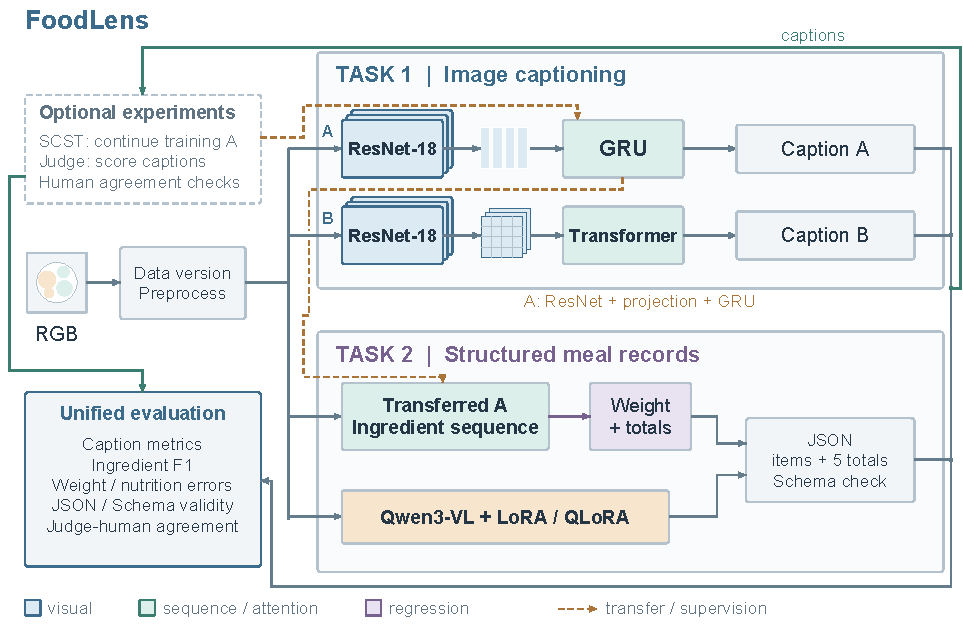
\includegraphics[width=\linewidth]{figures/architecture/figure06_system.pdf}
\caption{FoodLens 总体架构。实线表示数据流，虚线表示参数迁移或离线监督关系；两项任选实验复用描述模型及其输出。}
\label{fig:fl-system}
\end{figure}

共享数据层负责图文匹配、固定划分、文本编码和批处理，评价层接收按样本 ID 保存的预测文件，统一计算指标。任务一输出 Caption；任务二自主模型输出食材名称序列、对应重量与五维整餐数值，经确定性程序组装 JSON。Qwen3-VL 直接生成 JSON 文本，两条路线共用解析、Schema 校验与数值评价程序。该组织方式将模型能力与输出格式处理分开，便于追踪食材识别、定量估计和结构错误。

\subsection{食物图像描述生成模型设计}
\textbf{共享输入与文本表示。}两种自主模型均输入 $224\times224$ RGB 图像，使用 ImageNet 预训练 ResNet-18 的 \texttt{layer4} 输出 $F\in\mathbb{R}^{512\times7\times7}$，移除分类层\footnote{骨干输出位置与预处理依据 \href{https://docs.pytorch.org/vision/main/models/generated/torchvision.models.resnet18.html}{Torchvision ResNet-18 文档及其源码}。}。验证、测试采用短边缩放至 256 后中心裁剪，训练仅增加水平翻转，沿用预训练均值与标准差。两模型共享仅由训练 Caption 拟合的英文词级词表和规范化规则，保留标点，设置 \texttt{PAD/BOS/EOS/UNK}；最大生成长度初设为 64 Token，截断比例在训练前检查。以下维度和超参数均为起始配置，由验证集调整。


\textbf{模型 A：全局视觉条件的 GRU。}令 $v=\operatorname{GAP}(F)\in\mathbb{R}^{512}$，投影为 $z=\tanh(W_vv+b_v)\in\mathbb{R}^{256}$。采用 256 维词嵌入、单层 256 维 GRU，将 $z$ 同时作为初始隐藏状态和每步输入条件：
\begin{equation}
 h_0=z,\quad h_t=\operatorname{GRU}([E(y_{t-1});z],h_{t-1}),\quad
 p_\theta(y_t\mid y_{<t},I)=\operatorname{softmax}(W_oh_t+b_o).
 \label{eq:fl-gru}
\end{equation}
全局向量持续参与解码，降低长序列中视觉条件衰减的影响；输入拼接后的维度固定为 512，便于任务二直接复用 GRU 权重。

\begin{figure}[!ht]
\centering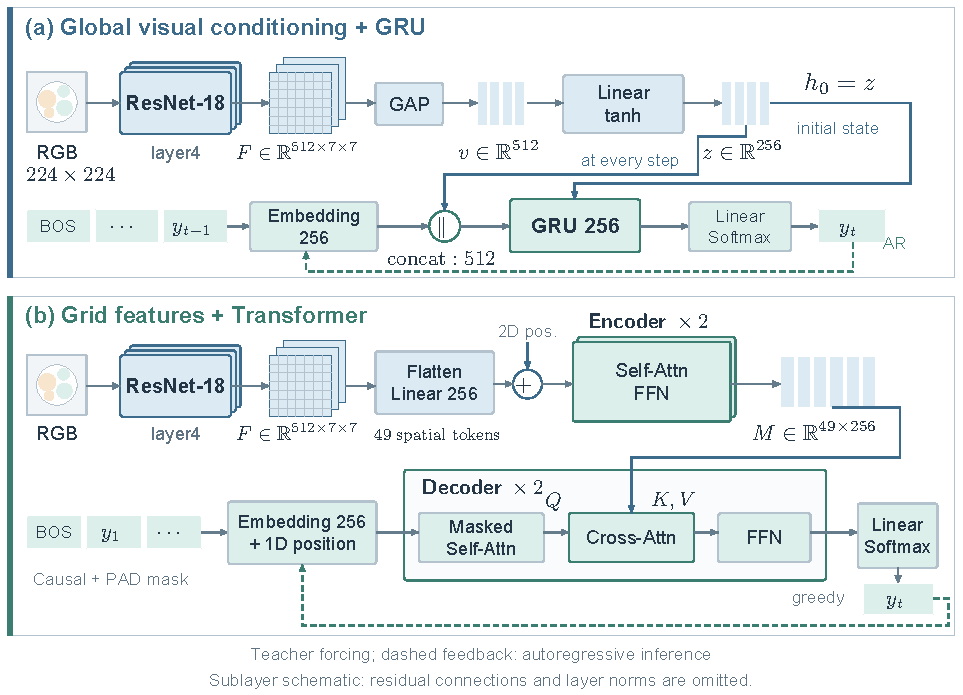
\includegraphics[width=\linewidth]{figures/architecture/figure07_caption.pdf}
\caption{任务一双模型内部结构。A 以全局条件驱动循环生成；B 保留 49 个空间位置，通过视觉自注意力及解码交叉注意力读取图像。训练输入为右移真实序列，推理输入为已生成前缀。}
\label{fig:fl-caption}
\end{figure}

\textbf{模型 B：网格视觉与 Transformer。}将 $F$ 展平为 $49\times512$，逐位置线性映射到 $d=256$，加上二维行列正弦位置编码，再由两层 Transformer Encoder 输出视觉记忆 $M\in\mathbb{R}^{49\times256}$。Decoder 初设两层、4 个注意力头、前馈维度 1024、Dropout 0.1，文本嵌入加一维位置编码。每层先执行因果自注意力，再以文本状态为 Query、$M$ 为 Key/Value 执行交叉注意力；每头维度为 64。固定大小网格无需视觉 Padding Mask，文本 Padding Mask 排除补齐位置；上三角因果掩码屏蔽未来 Token。该结构借鉴网格关系建模思路\cite{zeng2022s2}，不引入伪区域或多层网状连接。

\textbf{训练与解码。}Teacher Forcing 输入 $[\mathrm{BOS},y_1,\ldots,y_{T-1}]$，目标为 $[y_1,\ldots,y_{T-1},\mathrm{EOS}]$；交叉熵按全批非 PAD 目标数归一化，EOS 参与损失。先冻结骨干并保持 BatchNorm 为评价模式，训练投影与解码器；收敛后视验证结果以较小学习率解冻 \texttt{layer4}。主对照统一采用贪心生成，遇 EOS 或长度上限终止，束搜索仅作同协议补充。A 与 B 同时改变视觉表示和解码器，另设 B-Global：保留 B 的编码、解码配置，以投影全局向量形成单个视觉 Token，用一次轻量消融分析空间信息贡献。


\subsection{结构化膳食记录生成}
\subsubsection{自主混合预测架构与参数迁移}
任务二采用\textbf{共享视觉编码、食材序列生成、边界位置重量回归和整餐数值回归}的多任务结构，如图\ref{fig:fl-hybrid}。从任务一 A 的最优监督 Checkpoint 迁移 ResNet-18、$W_v,b_v$ 和 GRU；新增重量与营养回归头。食材序列使用与任务一相同的词级切分规则，在原词表后追加任务二训练集词语和边界 Token \texttt{SEP}，按 Token 字符串复制已有嵌入和输出层行，新行随机初始化。保留原词表 ID，验证集和测试集不参与扩词。这样既保留语言参数，也明确迁移范围。

\begin{figure}[!t]
\centering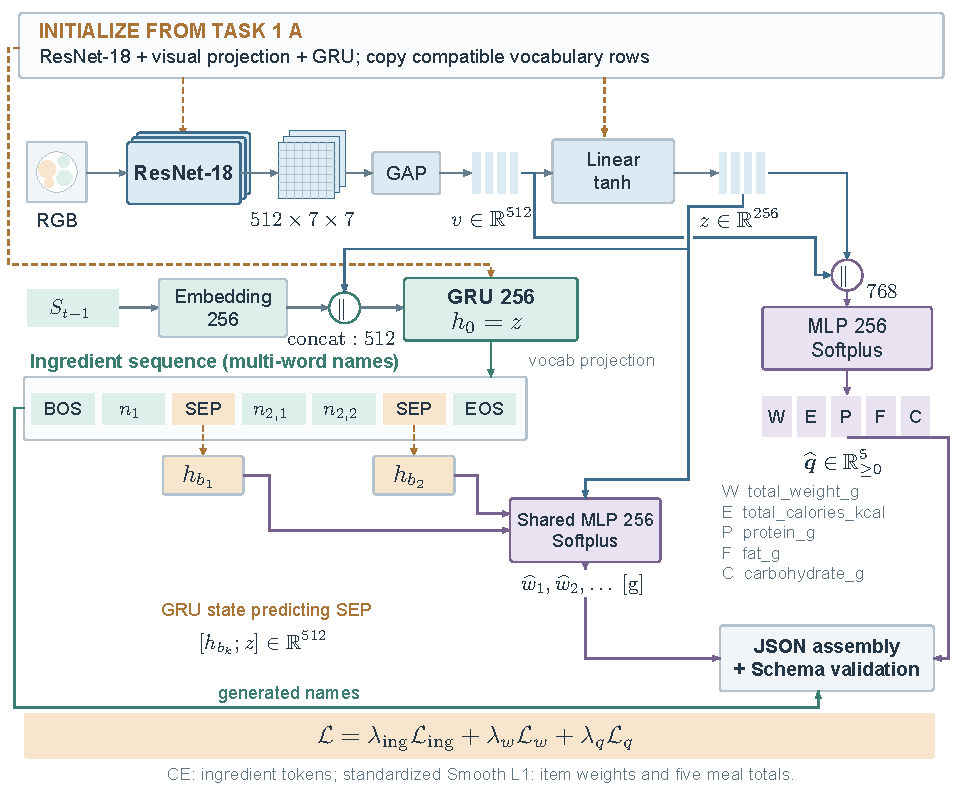
\includegraphics[width=\linewidth]{figures/architecture/figure08_hybrid.pdf}
\caption{任务二自主混合架构。第 $k$ 个 SEP 的预测状态 $h_{b_k}$ 来自产生该 SEP logits 的 GRU 隐藏状态，虚线按边界位置选取；整餐五维数值由独立分支预测。虚线为迁移或监督，推理时沿实线动态组装记录。}
\label{fig:fl-hybrid}
\end{figure}

\textbf{食材列表序列化。}名称先执行 Unicode 规范化、小写化与空白合并，不做基于测试标签的同义词扩展。同一记录中相同规范化名称合并并累加重量，再按名称字典序排序，得到 $K$ 项 $\{(n_k,w_k)\}_{k=1}^K$。监督序列为
\begin{equation}
 S=[\mathrm{BOS},\operatorname{tok}(n_1),\mathrm{SEP},\ldots,
 \operatorname{tok}(n_K),\mathrm{SEP},\mathrm{EOS}].
 \label{eq:fl-items}
\end{equation}
每个名称可占多个词，SEP 标识完整名称结束，排序规则减少同一集合多种排列带来的监督歧义。食材分支仍按式\eqref{eq:fl-gru}逐词生成；不以训练食材全名白名单约束解码，以允许已知词组成新名称。全新词映射至 UNK，含 UNK 的项记为识别失败；即便后续改用子词编码，开放名称的可表示性也需与视觉识别准确性分别验证。


\subsubsection{食材边界对齐与多任务训练}
\textbf{逐食材重量。}定义 $b_k$ 为目标 SEP 在预测序列中的时间步，$h_{b_k}$ 表示\emph{产生该 SEP 的 logits 所用状态}。Teacher Forcing 时该状态已读取完整的第 $k$ 个真实名称；批处理额外保存 $b_k$、$w_k$ 与有效项掩码，按位置 Gather 隐藏状态，不对 PAD 或普通词位置计算重量损失。推理每产生一个 SEP，便从同一位置提取状态并回归一项重量，输出项数由生成边界动态决定：
\begin{equation}
 \widehat w_k=\operatorname{softplus}(f_w([h_{b_k};z])),\qquad
 \widehat{\boldsymbol q}=\operatorname{softplus}(f_q([v;z]))\in\mathbb{R}_{\geq0}^{5}.
 \label{eq:fl-regression}
\end{equation}
两个 $f$ 为独立的两层 MLP，隐藏维度初设为 256。$\boldsymbol q$ 按固定顺序表示总重量、总热量、蛋白质、脂肪和碳水化合物，分别以 g、kcal、g、g、g 为单位。输出经 Softplus 保证非负，整餐头不依赖生成的食材前缀，避免名称错误直接阻断全部数值输出。

\textbf{尺度与联合目标。}以训练集估计逐项重量及每个整餐字段的均值 $\mu_j$、标准差 $s_j$，将 $s_j$ 下限设为 $10^{-6}$。模型先输出原单位非负值，再以 $\mathcal N_j(a)=(a-\mu_j)/s_j$ 同时变换预测和标签，计算尺度一致的 Smooth L1（阈值 1）：
\begin{align}
 \mathcal L_{\rm ing}&=-\frac{1}{N_{\rm tok}}\sum_{i,t}m_{it}
       \log p_\theta(S_{it}\mid S_{i,<t},I_i),\notag\\
 \mathcal L_w&=\frac{1}{N_{\rm item}}\sum_{i,k}a_{ik}
   \ell\bigl(\mathcal N_w(\widehat w_{ik}),\mathcal N_w(w_{ik})\bigr),\notag\\
 \mathcal L_q&=\frac{1}{5B}\sum_{i=1}^{B}\sum_{j=1}^{5}
   \ell\bigl(\mathcal N_j(\widehat q_{ij}),\mathcal N_j(q_{ij})\bigr),\notag\\
 \mathcal L&=\lambda_{\rm ing}\mathcal L_{\rm ing}+\lambda_w\mathcal L_w+
       \lambda_q\mathcal L_q.\label{eq:fl-joint}
\end{align}
其中 $m_{it}$ 排除 PAD，$a_{ik}$ 标识真实食材，$N_{\rm tok}$、$N_{\rm item}$ 为相应有效数，$B$ 为批大小；无有效项时重量损失置零。三个权重先取 1，观察各损失及梯度量级，仅在验证集上小范围调整。训练先冻结视觉骨干联合学习新任务，再按需解冻末级视觉层。重量监督使用真实名称条件，最终评价使用自由生成结果，二者差异作为误差传播分析的一部分。

\textbf{JSON 组装。}推理限制首项非空、SEP 前至少有一个名称词、EOS 只出现在列表边界；达到长度或项数上限时丢弃未闭合末项并记录截断。空名、UNK 和非有限重量进入失败记录；有效重复名称按名称合并、重量求和。输出根对象含 \texttt{items} 及五个数值字段，项对象仅含 \texttt{name}、\texttt{weight\_g}；验证字段集合、非空字符串、数值类型、有限性与非负性，拒绝布尔值和额外字段。组装时统一保留一位小数，数值评价使用同一交付值。依据已有审计，食材重量之和与整餐重量分别学习，\textbf{不设置二者相等的约束}。原始输出、清理日志与最终 JSON 同时留存，便于区分生成和后处理收益。


\subsubsection{Qwen3-VL 的领域参数高效适配}
预训练路线采用 \textbf{Qwen3-VL-4B-Instruct}，使用其官方 Processor 和 Chat Template 组织图像与对话\footnote{输入格式及微调入口参考 \href{https://huggingface.co/Qwen/Qwen3-VL-4B-Instruct}{官方模型卡}与 \href{https://github.com/QwenLM/Qwen3-VL}{Qwen3-VL 官方仓库}，实施时固定版本与模型 revision。}。每个样本的 user 消息包含 RGB 图像、固定膳食记录指令、字段与单位说明；assistant 消息为统一序列化的目标 JSON。仅 assistant 目标及其结束标记参与自回归交叉熵，系统提示、user 内容、图像占位和 PAD 的标签置为忽略值。训练前在单样本上逐段检查掩码，保留多模态控制 Token，序列超限时先控制图像 Token 与长度，不截断监督 JSON。

\begin{figure}[!t]
\centering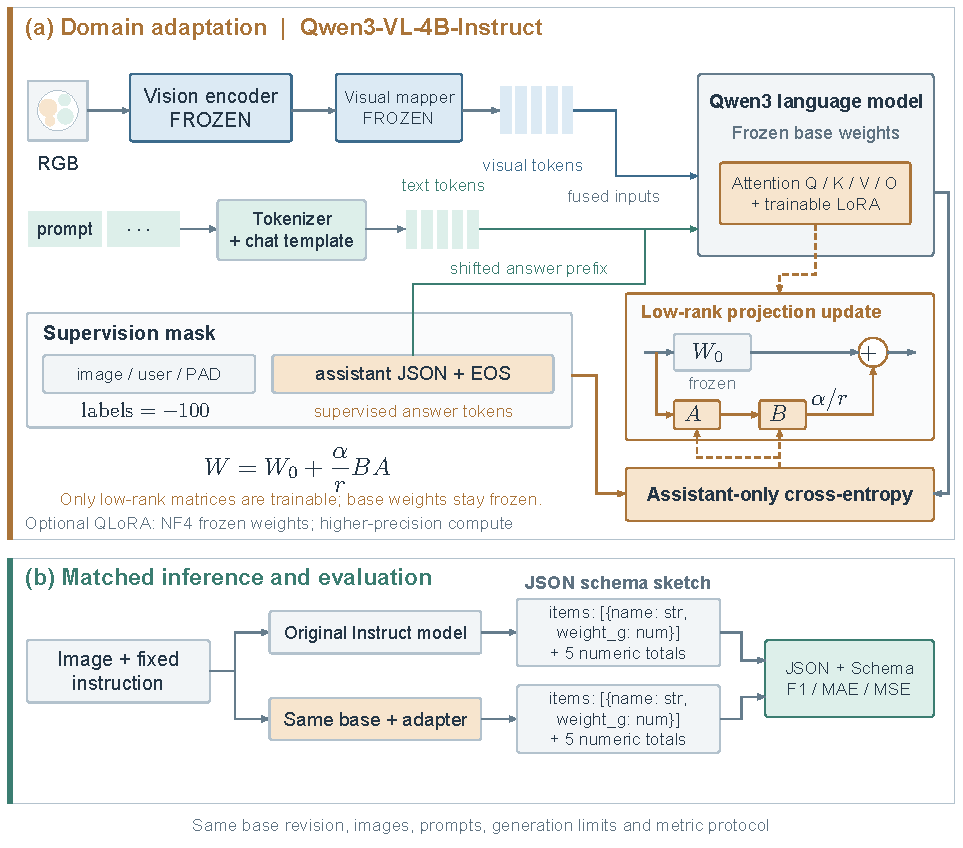
\includegraphics[width=\linewidth]{figures/architecture/figure09_qwen.pdf}
\caption{Qwen3-VL 领域适配流程。仅目标回答参与监督；同一基础模型在相同输入、生成和评价协议下比较适配前后差异。量化为可选存储策略，视觉部分初始冻结。}
\label{fig:fl-qwen}
\end{figure}

\textbf{适配与资源控制。}初始冻结视觉编码器、视觉语言映射及语言基础权重，在语言模型注意力的 Q/K/V/O 线性投影中注入 LoRA\cite{hu2022lora}，初设 $r=8$、$\alpha=16$、Dropout 0.05。依据模型实际模块路径限定注入范围，并输出可训练参数清单，避免同名视觉层被误选。先做小批量显存试跑：常规 BF16 LoRA 能容纳目标序列则优先采用；空间不足且算子兼容时，采用 NF4 4-bit、双重量化的 QLoRA\cite{dettmers2023qlora}，冻结量化权重，以 BF16 或硬件支持的计算精度训练适配器。配合梯度累积、梯度检查点和图像分辨率上限控制开销，保持任务目标不变。

主实验比较同一 4B revision 的原始 Instruct、领域微调版本及自主混合模型；若 24 GB 单卡环境无法稳定运行，成对切换到同一 2B 基础模型重新比较，单独报告规模。图像预处理、固定指令、最大输出长度及贪心解码在适配前后保持一致。生成文本先严格解析再校验 Schema，主指标不做提示重试或内容修复；失败样本进入全样本统计。保存原始字符串、错误类型与成功解析值；如附加格式修复实验，单列其结果。模型、适配器、Processor、量化配置和解码配置共同构成可复现的推理版本。


\subsection{训练优化与多模态评价}
\subsubsection{从监督训练衔接 SCST}
任选优化优先用于任务一模型 A。先按验证集 CIDEr-D 选定交叉熵训练 Checkpoint，再复制该权重进入低学习率 SCST 阶段\cite{rennie2017scst}。对同一训练图像，生成采样序列 $y^s\sim p_\theta$ 和贪心序列 $y^g$，使用训练参考描述计算 CIDEr-D 奖励 $r$：
\begin{equation}
 \mathcal L_{\rm SCST}=-\operatorname{stopgrad}\bigl[r(y^s)-r(y^g)\bigr]
   \sum_{t\leq T_s}\log p_\theta(y^s_t\mid y^s_{<t},I).
 \label{eq:fl-scst}
\end{equation}
EOS 参与概率和，EOS 后的 PAD 不参与；采样与贪心分支采用一致的模型模式和最大长度，基线与奖励不反向传播。CIDEr-D 文档频率仅由训练参考预计算并固定，避免随小批次改变奖励标尺。训练初期可使用 $\mathcal L_{\rm mix}=(1-\eta)\mathcal L_{\rm CE}+\eta\mathcal L_{\rm SCST}$，$\eta$ 初设 0.5，再由验证稳定性决定是否调整。

最小交付为同一 A 模型监督训练前后两个版本、完全一致的测试解码与四项文本指标，并保存逐样本奖励及典型描述。除 CIDEr-D 外，同时检查 BLEU-4、METEOR、ROUGE-L 和食材幻觉，分析优化目标提升是否伴随细节与可读性的改变。若预算允许，增加相同步数继续交叉熵的对照，以区分额外训练与奖励优化的作用。

\subsubsection{固定协议的 VLM-as-Judge 与人评对照}
评价借鉴 CLIPScore 的图文相容性\cite{hessel2021clipscore}以及 FLEUR、EXPERT 的视觉条件评分和解释组织\cite{lee2024fleur,kim2025expert}。使用冻结的原始 Instruct VLM 作 Judge，独立于领域微调权重；输入仅为图像、候选 Caption 和固定评分标准，隐藏模型名称及参考描述。四维均采用 1--5 分，语义正确性检查主要菜品与关系，细节覆盖检查可见属性，事实可靠性以高分表示少幻觉与错误食材，语言流畅度检查语法及自然程度。每维同时输出一句图像证据，固定模型 revision、提示模板、温度 0 与解析规则，解析失败率另行报告。

初始从测试集固定抽取约 60 张图像，覆盖菜品类别、长短描述与困难样本；在查看模型结果前锁定样本 ID。比较 A、B、A+SCST 的同图输出，以随机顺序、匿名方式交给两名组员独立评分，少量分歧样本由第三名组员讨论裁定。用 Spearman 相关衡量 Judge、传统指标与人工均分的一致性，按图像进行 Bootstrap 给出区间，另报两名人评的加权 Cohen $\kappa$。人工样本较少时以维度趋势和错误案例为主；Judge 使用固定评分协议，不训练专门评价模型。记录同系列模型可能带来的偏好，并保留与人评不一致的原始解释供复核。


\FloatBarrier
\subsection{数据处理与实验设计}
\textbf{Food-500 Cap 的可靠映射与划分。}官方说明将数据分为 19,760 条训练和 4,940 条测试图文对\cite{ma2023food}；本地标注文件实际为 19,880 和 4,940 条，须记录这一版本差异。本地图片来自社区镜像，先以官方 \texttt{filename}、类别与镜像索引建立显式映射，以官方 Caption 为文本依据；无法唯一确认的映射排除并记录，图像解码失败单列。复用已有审计结论处理少量缺失、映射差异及重复图像，固定文件 SHA-256、数据源 revision、排除原因和最终样本清单，不凭行号直接拼接图文。

对于跨官方训练/测试的相同图像组，测试归属优先，移除训练侧副本；同一测试重复组仅保留稳定排序后的一个代表。近重复组复核后采用相同策略。再按重复组从剩余官方训练集划出约 10\% 验证样本，以类别分层尽量保持分布，种子设为 42；组内样本不跨划分。清洗后的计数以 manifest 为准，与原始数量分别报告。词表、长度统计及 SCST 奖励统计均仅从最终训练集拟合。

\textbf{结构化数据与输入隔离。}本地 \texttt{nutrition5k-student-v1} 包含 Train 2,338、Validation 414、Test 506，共 3,258 条，保留学校原始划分。数据加载器将 \texttt{image} 与 \texttt{target} 分开返回，推理接口只允许图像及固定指令，禁止传入 \texttt{target\_text} 和含答案的 \texttt{metadata}。已有审计发现可变项数、训练未见食材、总量不一致及少量疑似同餐跨划分，故主结果沿用原划分，并在已标记疑似组上附分层敏感性分析。所有阈值、规范化映射与模型选择均在训练/验证阶段确定，测试集仅用于冻结方案后的最终评价。

\begin{table}[!htbp]
\caption{统一评价协议与失败样本计入方式}
\label{tab:fl-metrics}\centering\small
\setlength{\tabcolsep}{4pt}\renewcommand{\arraystretch}{1.15}
\begin{tabularx}{\linewidth}{@{}P{2.35cm}YP{4.0cm}@{}}\toprule
\textbf{对象} & \textbf{主要指标与统计单位} & \textbf{协议要点}\\\midrule
Caption & BLEU-4、METEOR、ROUGE-L、CIDEr-D；语料级得分 & 同一 Tokenizer、单参考、实现版本与缩放单位\\
食材名称 & Micro F1 为主，Macro F1 为辅；见过/未见名称分层 & 规范化全名精确匹配，预测无效项计 FP\\
食材重量 & 匹配项 MAE/MSE；全名称并集 MAE/MSE & 漏检与多检按另一侧重量为零计入\\
整餐五维 & 各字段原单位 MAE、MSE，逐字段报告 & 解析失败采用预先规定的零预测计误差\\
输出结构 & JSON 语法合法率、Schema 有效率 & 分母均为全部样本；额外报告截断/失败率\\\bottomrule
\end{tabularx}
\end{table}

\textbf{名称匹配与重量误差。}真实和预测项采用同一名称规范化及重复项合并。按全名精确匹配，不用重量进行匹配，避免利用数值标签挑选最有利配对。令 $U_i$ 为两侧名称并集，缺失侧重量置零，定义
\begin{equation}
 E_{\rm union}^{(p)}=\frac{\sum_i\sum_{n\in U_i}|\widehat w_i(n)-w_i(n)|^p}
 {\sum_i|U_i|},\qquad p=1,2.\label{eq:fl-union}
\end{equation}


式\eqref{eq:fl-union}分别为并集 MAE 和 MSE，同时惩罚漏检和多检。匹配项误差单列，并给出匹配覆盖率；无匹配项记为不可计算，不记为零误差。非法名称项保留为互不匹配的预测项，计 FP 及其可读重量误差；完全无法解析的输出视作空食材集合、整餐零预测，仍保留在全样本分母中。另报有效输出子集误差与覆盖率，解释零预测约定的影响。对未见名称分别统计全名与组成词是否在训练集出现。辅助文本指标可用于规范化食材序列或 JSON，但不替代名称、重量及结构评价。

\begin{table}[!htbp]
\caption{按实施优先级组织的最小实验矩阵}
\label{tab:fl-experiments}\centering\small
\setlength{\tabcolsep}{4pt}\renewcommand{\arraystretch}{1.13}
\begin{tabularx}{\linewidth}{@{}P{1.55cm}P{4.6cm}Y@{}}\toprule
\textbf{层次} & \textbf{实验组} & \textbf{主要问题}\\\midrule
必选一 & A、B；共享划分与贪心解码 & 全局循环与网格注意力两条路线的总体差异\\
必选二 & 自主混合；同规模原始/微调 Qwen & 食材、定量与结构质量的领域适配收益\\
轻量消融 & B-Global；混合模型仅视觉迁移 vs. 视觉+GRU 迁移 & 空间信息贡献、序列迁移是否有效\\
任选 & A 的 CE vs. SCST；Judge 与双人人评 & 奖励优化收益、评分一致性与幻觉变化\\\bottomrule
\end{tabularx}
\end{table}

主对照固定清洗版本、训练预算与选择规则，记录参数量、可训练参数、单图推理耗时和实际显存。自主模型在预算允许时使用三个种子，报告均值与标准差；VLM 优先完成一个固定种子的配对适配实验，明确重复次数。任务一按验证 CIDEr-D 选模型；任务二按验证 Micro F1 选模型，接近时比较五维标准化 MAE，再比较有效率，规则在测试前固定。误差分析覆盖可见/隐含食材、长列表、未见名称、大份量、疑似同餐样本及重度质量不守恒样本，不将这些标记作为推理输入。

\subsection{工程实现与可行性分析}
采用 PyTorch 与 Torchvision，自主编写条件生成、掩码、损失、解码、边界对齐与记录组装；Transformer 可复用标准层，VLM 使用 Transformers、PEFT 和兼容的量化后端。工程拆分为数据与 manifest、Tokenizer、视觉骨干、序列解码器、回归头、训练器、解码器、Schema 与指标模块。训练接口接收图像及监督，返回分项损失；推理接口只接收图像和配置，返回逐样本预测及状态。先用 CPU 小样本验证尺寸、因果掩码、边界 Gather、梯度流、非负输出与 JSON 往返，再进入 GPU 训练。

配置统一保存种子、数据哈希、词表、数值统计、模型维度和生成参数；Checkpoint 保存模型、优化器、调度器、随机数状态及版本信息。自主模型初设 AdamW、学习率 $3\times10^{-4}$、梯度裁剪 1.0；视觉层解冻后使用主学习率的十分之一，采用验证早停。总算力预算约 300 元，计划单卡 24 GB，先完成两项必选任务及同规模微调对照，再复用已有模型开展任选实验。GPU 型号、LoRA/QLoRA 最终配置、批量与步数由小样本试跑和预算共同确定，不预设训练时长或峰值显存。

主要风险集中在 RGB 份量歧义、小数据过拟合、食材序列训练与自由生成的差异，以及多模态量化兼容性。通过冻结骨干、验证早停、全样本指标和输出追踪控制风险；主混合分支若难以收敛，回退到共享 ResNet 的多标签食材预测加数值回归，并保留回退原因。优先交付可复现的完整推理与评价链路，再增加网格交叉注意力等局部增强。上述设计为待实施方案，模型效果及资源数据均由后续实验给出。

\clearpage
\setcounter{section}{6}
\fancyhead[R]{\small\color{FLMid} 组员分工及检查点}
\section{组员分工及检查点}
\label{sec:team}
\subsection{模块责任与协作方式}
三人分别承担自主模型、数据与适配实验、评价与分析，交付可运行模块及验证记录。罗开炜统筹集成，各模块由负责人实施、另一成员复核。

\begin{table}[!ht]
\caption{模块负责人、独立成果与交叉复核}
\label{tab:member-roles}\centering\small
\setlength{\tabcolsep}{4pt}\renewcommand{\arraystretch}{1.13}
\begin{tabularx}{\linewidth}{@{}P{1.35cm}YP{4.35cm}@{}}\toprule
\rowcolor{FLBlue!8}\textbf{成员} & \textbf{主责与独立技术成果} & \textbf{交叉复核}\\\midrule
\textbf{\color{FLBlue}罗开炜} & A/B/B-global、自主训练器、Hybrid 迁移与 SCST；训练恢复、推理接口及技术集成。 & 郝天乐复跑命令；张嘉荣核对模型图和对照。\\\addlinespace
\textbf{\color{FLTeal}郝天乐} & 数据审计、manifest、统一指标、GPU 排期；Qwen 数据处理、LoRA 训练与配对评测。 & 罗开炜审查监督掩码与适配范围；张嘉荣复算结果表。\\\addlinespace
\textbf{\color{FLAmber}张嘉荣} & 文献调研、Judge 接入与解析、人评协议、统计分析 Notebook；图表、报告与展示。 & 郝天乐复核统计输入与结果；罗开炜协助模型接入。\\\bottomrule
\end{tabularx}
\end{table}

郝天乐与张嘉荣独立盲评，罗开炜复核分歧。先以非测试样本校准标准，再锁定规则；正式评分隐藏候选来源及 Judge 结果。原始独立评分用于人评一致性与人工均分，协商裁定仅用于案例解释。抽样和统计协议与第五章一致。

\subsection{个人交付与可度量检查点}
各阶段按“产物、运行记录、通过条件、复核人”验收。表~\ref{tab:member-checks}明确个人成果，不以提交配置替代运行证据。
\begin{table}[!ht]
\caption{个人阶段交付与验收条件}
\label{tab:member-checks}\centering\small
\setlength{\tabcolsep}{4pt}\renewcommand{\arraystretch}{1.13}
\begin{tabularx}{\linewidth}{@{}P{2.15cm}YYY@{}}\toprule
\rowcolor{FLBlue!8}\textbf{检查点} & \textbf{\color{FLBlue}罗开炜} & \textbf{\color{FLTeal}郝天乐} & \textbf{\color{FLAmber}张嘉荣}\\\midrule
\textbf{开题}\newline 11 月 15 日 & 模型与接口表，明确输入、输出、迁移范围及选模依据。 & 数据来源与计数核验，图文映射、重复组及排除项审计办法。 & 文献与研究问题对应表，开题稿及课程任务覆盖核对。\\\addlinespace
\textbf{中期}\newline 12 月 6 日 & A/B 训练推理与 Hybrid 原型；郝天乐加载 A 权重复跑真实样本。 & manifest、哈希、GPU 试跑及四指标；预测 ID 与清单逐项对应。 & 独立复算指定指标并核对总表；同图案例、中期材料及人评草案。\\\addlinespace
\textbf{实验合并}\newline 12 月 25 日 & 迁移、SCST/等步数 CE 权重与验证记录；冻结测试版本。 & Qwen 配对结果和失败统计；罗开炜复跑适配器并核验监督范围。 & Judge、双人原始评分与统计 Notebook；郝天乐复算一致性及相关性。\\\addlinespace
\textbf{结题}\newline 1 月 17 日 & 核对代码、权重及配置；审查复现记录，统一提交。 & 全量预测、指标与资源记录；配合跨成员复算并解释差异。 & 报告及幻灯片或视频；独立运行演示，核对图表出处。\\\bottomrule
\end{tabularx}
\end{table}

\textbf{阶段牵头与交接。}开题、中期、结题分别由张嘉荣、郝天乐、罗开炜牵头，组长经教学云平台统一提交。每周核对进度，郝天乐登记 GPU 作业。交接包含代码版本、配置、数据哈希、命令、预测及失败统计；接收人核验 ID 全集与分母、复算指标。接口变动经交叉复跑后合并，阻塞时组长安排协助。


\clearpage
\fancyhead[R]{\small\color{FLMid} 项目时间安排}
\section{项目时间安排}
\label{sec:schedule}
项目按“数据审计、Caption 训练与指标、任务二迁移、Qwen 配对实验、SCST 与 Judge”推进，每阶段完成可运行入口及验收记录后进入下一阶段。图~\ref{fig:team-timeline}给出初始排期；模型接口开发、文档与离线复核并行，正式 GPU 作业按依赖顺序执行。当前已有 CPU tiny 链路，正式训练入口和 GPU 效果仍待验证，以下日期属于计划检查点。

\begin{figure}[!ht]
\centering% Weekly task windows; final evaluation dependencies are expanded below.
\begin{tikzpicture}[x=1.24cm,y=-1cm,font=\fontsize{8}{10}\selectfont]
\foreach \x/\lab in {0/11.04,1/11.09,2/11.16,3/11.23,4/11.30,5/12.07,6/12.14,7/12.21,8/12.28,9/01.04,10/01.11}{
 \node[text=FLBlue,font=\fontsize{7.5}{9}\selectfont] at (\x+.5,0) {\lab};
 \draw[FLLine!45] (\x,.23) -- (\x,4.7);}
\draw[FLLine!45] (11,.23)--(11,4.7);
\foreach \y/\lab/\clr in {.8/罗开炜/FLBlue,1.85/郝天乐/FLTeal,2.9/张嘉荣/FLAmber,3.95/GPU/FLMid}{
 \fill[\clr!4] (0,\y-.44) rectangle (11,\y+.44);
 \node[anchor=east,text=\clr,font=\small\bfseries] at (-.12,\y){\lab};}
\def\slot#1#2#3#4#5{\filldraw[rounded corners=1.7pt,draw=#4!70,fill=#4!10] (#1+.035,#3-.34) rectangle (#2-.035,#3+.34);
\node[text=FLText,align=center] at ({(#1+#2)/2},#3){#5};}
\slot{0}{2}{.8}{FLBlue}{方案与接口}
\slot{2}{4.45}{.8}{FLBlue}{训练器与模型联调}
\slot{4.45}{6.43}{.8}{FLBlue}{迁移开发\\适配复核}
\slot{6.43}{7}{.8}{FLBlue}{\fontsize{7}{9}\selectfont SCST}
\slot{7}{8}{.8}{FLBlue}{分歧\\复核}
\slot{8}{11}{.8}{FLBlue}{复现检查与技术整合}
\slot{0}{3}{1.85}{FLTeal}{数据审计、指标与试跑}
\slot{3}{5.57}{1.85}{FLTeal}{Caption 与迁移评测}
\slot{5.57}{7}{1.85}{FLTeal}{Qwen\\统一评测}
\slot{7}{8}{1.85}{FLTeal}{盲评\\复算}
\slot{8}{11}{1.85}{FLTeal}{误差分层与独立复算}
\slot{0}{2}{2.9}{FLAmber}{调研与开题}
\slot{2}{5}{2.9}{FLAmber}{分析工具、案例与中期材料}
\slot{5}{7}{2.9}{FLAmber}{Judge 接入\\人评校准}
\slot{7}{8}{2.9}{FLAmber}{盲评\\统计}
\slot{8}{11}{2.9}{FLAmber}{统计分析、展示与报告}
\slot{2.4}{3}{3.95}{FLMid}{\fontsize{7}{9}\selectfont 试跑}
\slot{3}{4.45}{3.95}{FLMid}{A/B\\含消融}
\slot{4.45}{5.57}{3.95}{FLMid}{Hybrid}
\slot{5.57}{6.43}{3.95}{FLMid}{Qwen}
\slot{6.43}{7}{3.95}{FLMid}{\fontsize{7}{9}\selectfont SCST\\\fontsize{7}{9}\selectfont +CE}
\slot{7}{8}{3.95}{FLMid}{测试生成\\Judge}
\node[flnote,text width=3.4cm,font=\fontsize{7.5}{9}\selectfont] at (9.5,3.95)
 {冻结配置下按需复跑\\离线分析不持续占用 GPU};
\foreach \x/\lab in {2/开题,5/中期,7/冻结,11/结题}{
 \fill[FLBlue] (\x,4.54)--(\x+.065,4.63)--(\x,4.72)--(\x-.065,4.63)--cycle;
 \node[anchor=north,text=FLBlue,font=\fontsize{7.5}{9}\selectfont] at (\x,4.75) {\lab};}

\node[fllabel,anchor=west] at (-1.12,5.5) {正式评价与汇报的先后关系};
\node[flnode,text width=2.55cm,minimum height=1.05cm] (freeze) at (.12,6.4)
 {\textbf{12/20}\\冻结模型与协议};
\node[flaccent,text width=2.55cm,minimum height=1.05cm] (generate) at (2.55,6.4)
 {\textbf{12/21 起}\\测试生成、Judge};
\node[flaccent,text width=2.55cm,minimum height=1.05cm] (human) at (4.98,6.4)
 {\textbf{12/22--24}\\双人独立盲评};
\node[fltrain,text width=2.55cm,minimum height=1.05cm] (merge) at (7.41,6.4)
 {\textbf{12/25}\\统计复核与合并};
\node[flnode,text width=2.55cm,minimum height=1.05cm] (present) at (9.84,6.4)
 {\textbf{12/26--28}\\演练与预留汇报};
\draw[flarrow] (freeze.east)--(generate.west);
\draw[flarrow] (generate.east)--(human.west);
\draw[flarrow] (human.east)--(merge.west);
\draw[flarrow] (merge.east)--(present.west);
\node[flnote,anchor=west,font=\fontsize{8}{10}\selectfont] at (-1.12,7.2)
 {盲评仅使用匿名候选；Judge 结果对评分者隐藏。图示为初始排期，依 GPU 试跑修订。};
\end{tikzpicture}


\caption{团队工作、单卡窗口与正式评价衔接。横轴为各周起始日期，1 月为 2027 年；菱形标记检查点。下方展开冻结、生成、盲评及合并顺序，GPU 行表示作业窗口而非持续占用。}
\label{fig:team-timeline}
\end{figure}

\textbf{11 月 4--22 日：方案、数据与运行条件就绪。}11 月 15 日完成开题提交；22 日前由郝天乐固定 Food500 图文映射、重复组、排除清单与划分，同时核验任务二原始数据。罗开炜实现自主训练器，郝天乐接入四指标，张嘉荣梳理文献依据并准备分析 Notebook。利用少量 GPU 时间预检查 Qwen 加载、监督掩码和适配器保存，检查 Judge 解析及 SCST 奖励接口，不将接口试跑作为正式实验结果。首次试跑记录批量、精度、峰值显存和吞吐，由郝天乐据此估算训练、生成及重跑时间，三人共同更新排期。

\textbf{11 月 23 日至 12 月 6 日：Caption 验收与中期原型。}单卡先完成 A/B 训练和统一四指标评价，再运行 B-global 消融；按验证 CIDEr-D 选定 A 权重。罗开炜并行准备迁移接口，取得正式权重后完成 Hybrid 原型，郝天乐复跑真实样本。12 月 3--5 日联调并交叉复算，张嘉荣整理同图案例与中期资料，6 日提交。中期验收要求真实数据链路、可加载权重、四指标及失败统计均可出示，不以 tiny smoke 替代正式原型记录。

\textbf{12 月 7--20 日：迁移、适配与奖励优化。}7--10 日完成 Hybrid 训练及两种迁移对照；11--16 日由郝天乐运行 Qwen 同规模原始/微调配对实验，罗开炜复核监督范围，张嘉荣在非测试样本上完善 Judge 和人评工具。17--20 日由罗开炜完成 SCST 与等步数继续交叉熵对照，郝天乐检查评价覆盖与训练记录。各模型均依据验证集选择；20 日统一冻结权重、数据版本、解码和评价协议，同时锁定人评样本 ID 与规则。

\textbf{12 月 21--28 日：正式评价、人工复核与展示。}21 日起生成冻结版本的测试预测和同图匿名候选，随后运行 Judge；22--24 日郝天乐与张嘉荣独立盲评，罗开炜复核分歧，张嘉荣汇总统计。按第五章约 60 张图像、A/B/A+SCST 三组输出估算，每名评分者需评价约 180 条描述，每条含四维评分及简短依据。25 日验收结果表、人评记录和可运行统计，26--27 日用于差异复核、展示整合与演练，28 日预留口头汇报。

\textbf{12 月 29 日至 1 月 17 日：分析与交付。}开展分层误差分析和独立复现，整理 Notebook/Markdown 报告及展示材料，1 月 14 日完成组内交付检查，15--16 日修正材料和复现说明，17 日统一提交。冻结后的测试结果仅用于评价与分析，不据此调整模型、提示或后处理；运行故障可按相同冻结配置重跑，并保留原因与日志。

\begin{table}[!ht]
\caption{共同里程碑与验收后交付}
\label{tab:project-schedule}\centering\small
\setlength{\tabcolsep}{4pt}\renewcommand{\arraystretch}{1.12}
\begin{tabularx}{\linewidth}{@{}P{2.0cm}P{1.65cm}Y@{}}\toprule
\textbf{日期} & \textbf{牵头人} & \textbf{交付条件}\\\midrule
11 月 15 日 & 张嘉荣 & 开题报告、研究问题、模型对照及个人检查点。\\
11 月 22 日 & 郝天乐 & 可追溯数据清单、指标预检查、GPU 试跑与修订排期。\\
12 月 6 日 & 郝天乐 & A/B 四指标、选定 A 权重、Hybrid 原型及中期资料。\\
12 月 20 日 & 罗开炜 & 计划实验的验证记录与选定权重，冻结测试和人评协议。\\
12 月 25 日 & 张嘉荣 & 统一结果表、Judge 与双人原始评分、可复算分析及展示版本。\\
1 月 14 日 & 罗开炜 & 跨成员复现通过，报告、展示材料与大文件获取说明齐备。\\
1 月 17 日 & 罗开炜 & Notebook/Markdown 报告，另交幻灯片或 2--5 分钟视频。\\\bottomrule
\end{tabularx}
\end{table}

\textbf{缓冲与延期处理。}11 月 22 日、12 月 6 日及 16 日检查关键路径。若数据映射或单卡吞吐不能支持原排期，由组长在下一次训练前更新作业顺序：保障两项必选及已选 SCST、Judge 的完整交付，优先调整额外种子、扩展消融与图表美化；保留约定的核心对照和失败统计。数据未锁定时继续接口及任务二数据核验，不启动未经审计的 Caption 正式训练。若核心实验仍延期，同步更新冻结和人评窗口，至少预留三天双人评分与一天统计复核；汇报如实区分已完成和待完成内容，不将未执行实验写成结果。

三次课程材料分别于 11 月 15 日、12 月 6 日及次年 1 月 17 日 24:00 前由组长提交。中期选择书面报告或口头报告；中期与结题口头汇报暂按 12 月 7 日和 12 月 28 日预留，具体形式及日期以教师最新通知为准。


\clearpage
\fancyhead[R]{\small\color{FLMid} 参考文献}
\par\FloatBarrier
\begingroup
\setstretch{1.02}\small
\setlength{\bibsep}{3pt}\interlinepenalty=10000
\renewcommand{\refname}{参考文献}
\bibliographystyle{bibliography/foodlens-unsrtnat}\bibliography{bibliography/references}
\endgroup
\end{document}
